\chapter{Meta-Learning}

\section{Introduction to Meta-Learning}

Traditional deep learning is designed to solve a single fixed task. A model is trained on a large labeled dataset containing predefined classes such as \textit{Dog}, \textit{Cat}, \textit{Bird}, and \textit{Horse}. During training, the model learns to recognize only these classes.

\begin{figure}[H]
\centering
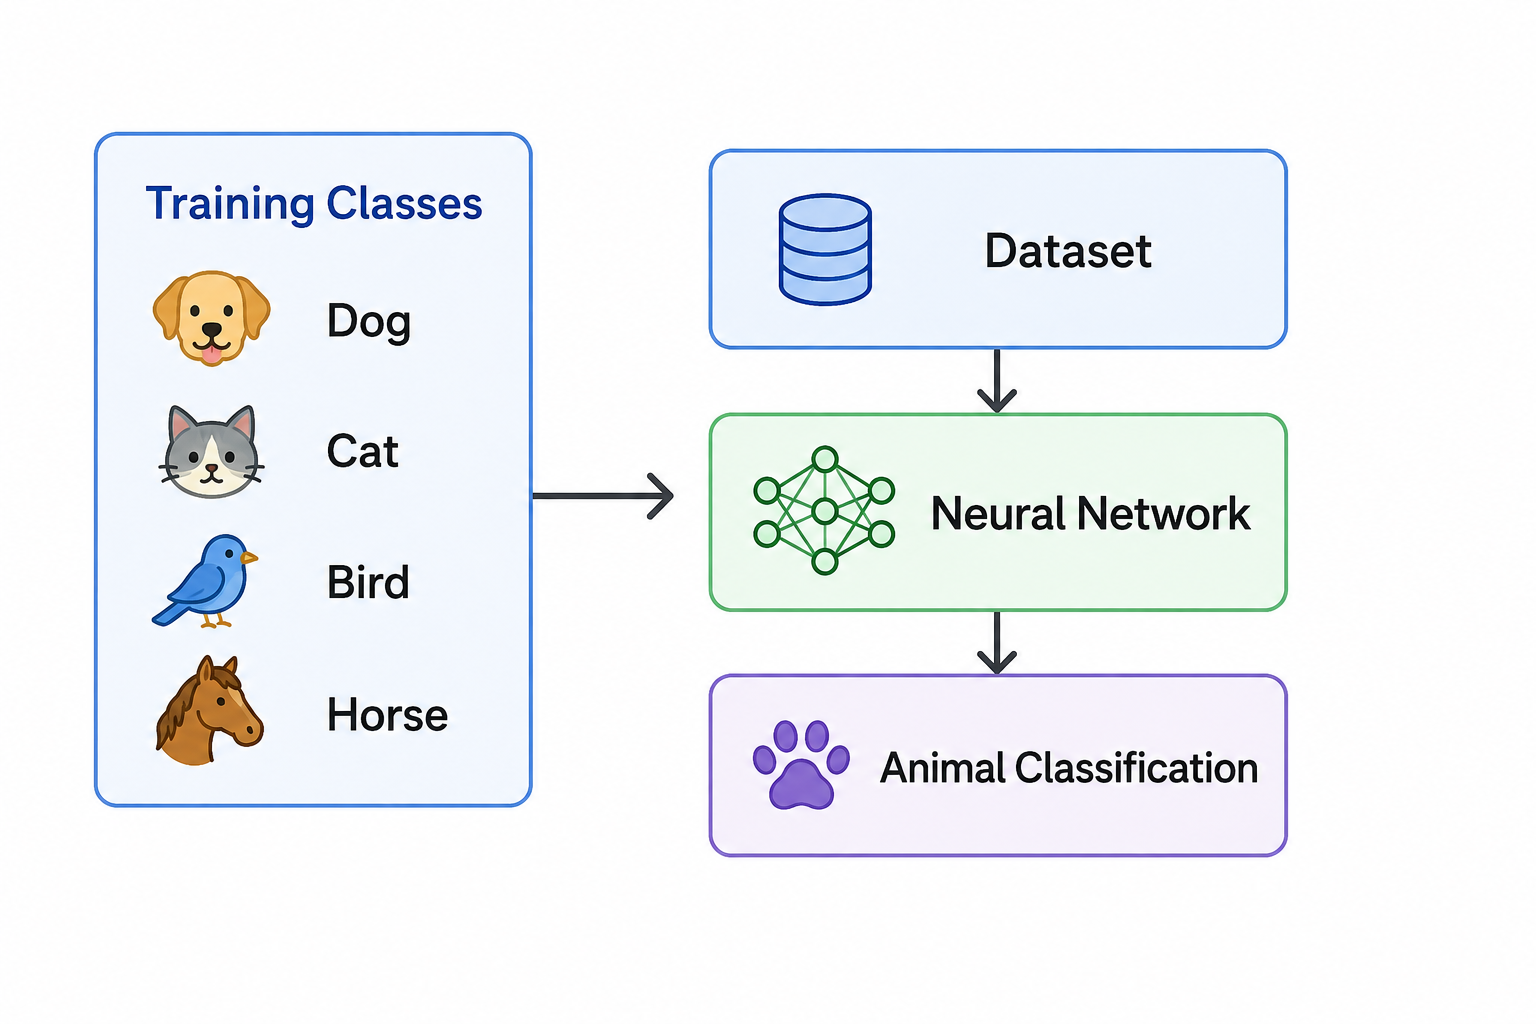
\includegraphics[width=0.85\textwidth]{figures/11-1 figure.png}
\label{fig:traditional_supervised_learning}
\end{figure}

After training, the model performs well on these known classes. However, when a new task introduces previously unseen classes, such as \textit{Camel} or \textit{Koala}, the model cannot recognize them effectively because it has never encountered these categories during training.

To adapt the model to the new task, it is typically necessary to:

\begin{itemize}
    \item Collect a large number of labeled examples for the new classes.
    \item Fine-tune or retrain the model using the new dataset.
    \item Repeat the training process whenever a new task is introduced.
\end{itemize}

Therefore, traditional deep learning is highly effective for solving a single predefined task, but it adapts slowly to new tasks or new classes because it requires substantial labeled data and additional training.

\subsection*{Can a Model Learn a New Task from 1 or 5 Examples?}

Humans can learn a new concept from seeing just one or two examples. They do not require thousands of observations. In contrast, traditional deep learning requires a fixed mapping from input to output, so the model cannot perform on a new task without acquiring labeled data and retraining or fine-tuning before it can perform.

\textbf{The Main Idea of Meta-Learning}:
Meta-Learning focuses on training across many tasks to learn how to quickly adapt to new tasks. Instead of optimizing the model for a single problem, it trains the model on many tasks so that it acquires a general learning strategy that can be used when encountering unseen tasks.

This is why Meta-Learning is called: \textbf{``Learning to Learn''}.

\begin{figure}[H]
\centering
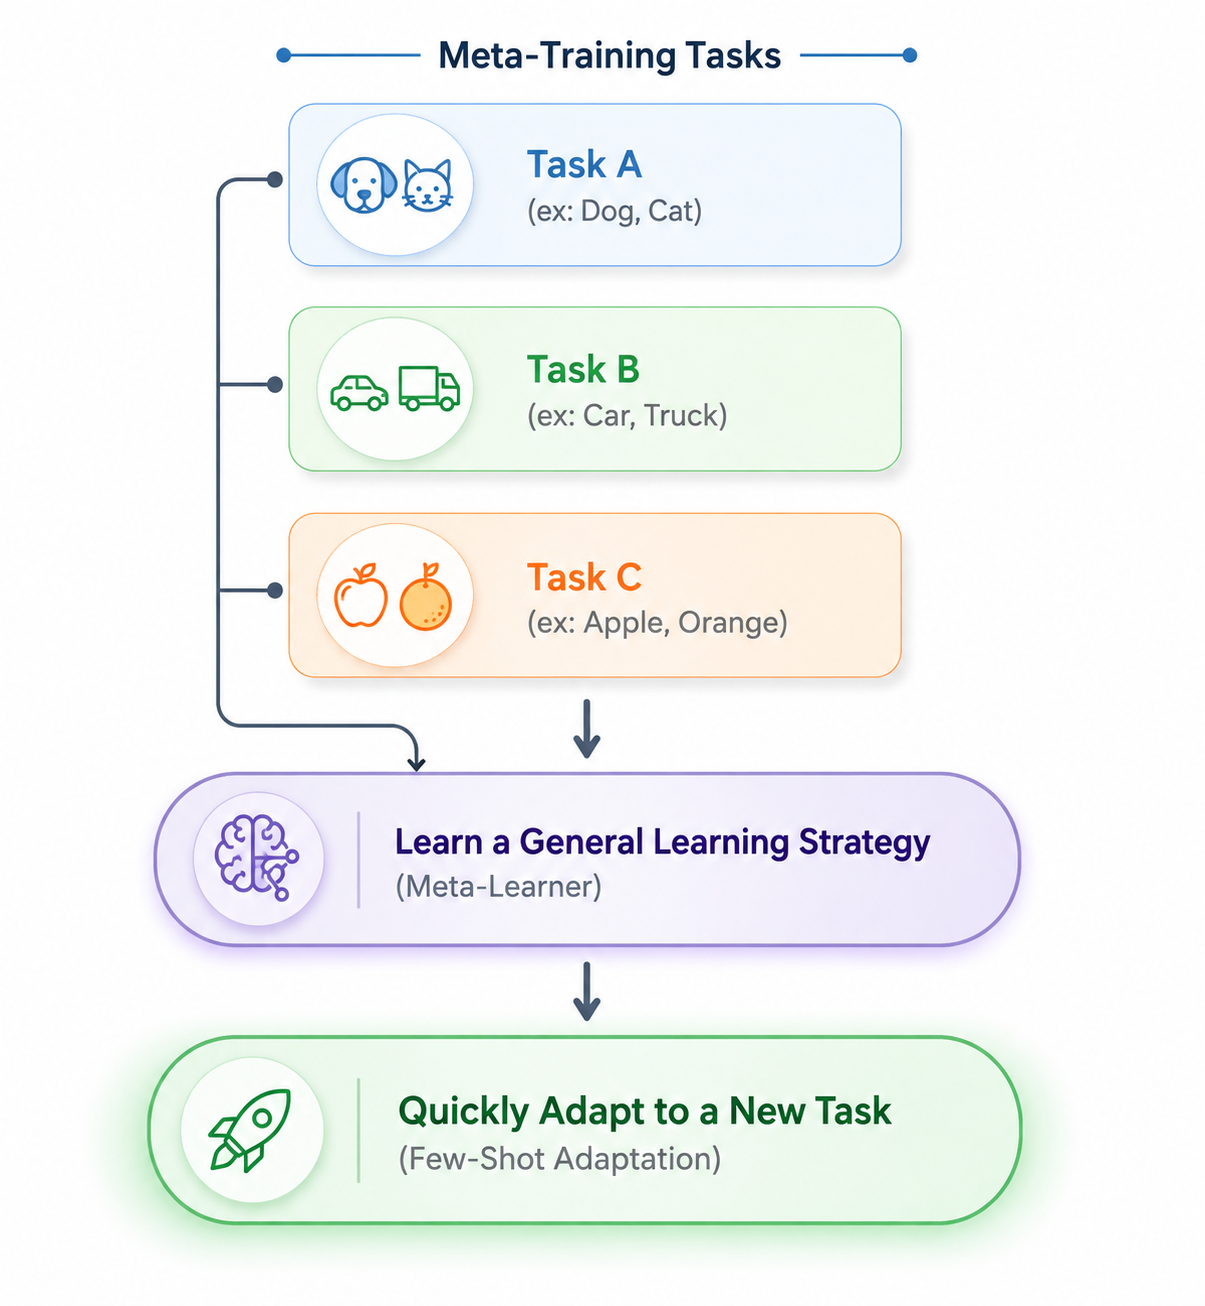
\includegraphics[width=0.85\textwidth]{figures/11-2 figure.png}
\caption{Meta-Learning Paradigm: Learning a General Strategy Across Multiple Meta-Training Tasks.}
\label{fig:meta_learning_concept}
\end{figure}

Unlike traditional deep learning which trains on one dataset for one task, Meta-Learning trains across many tasks:
\begin{itemize}
    \item \textbf{Task A} (ex: Dog, Cat)
    \item \textbf{Task B} (ex: Car, Truck)
    \item \textbf{Task C} (ex: Apple, Orange)
\end{itemize}

The model is trained on small tasks, not a single large dataset. Over time, it learns how to adapt quickly to new tasks independently.
The model continuously switches between tasks during training instead of training on one dataset. It learns patterns that help solve any new task.

\subsection*{Few-Shot Learning}

Meta-Learning is closely related to Few-Shot Learning:
\begin{itemize}
    \item \textbf{Zero-Shot}: No labeled examples of the target (new) classes.
    \item \textbf{One-Shot}: One labeled example per class.
    \item \textbf{Few-Shot}: A small number of labeled examples per class (typically 2--10).
    \item \textbf{Many-Shot}: Hundreds or thousands of labeled examples per class.
\end{itemize}

Traditional deep learning uses mini-batches. Instead, Meta-Learning training is divided into \textbf{episodes}:
\begin{itemize}
    \item \textbf{Episode 1}: Dogs, Cats
    \item \textbf{Episode 2}: Cars, Trucks
    \item \textbf{Episode 3}: Flowers
    \item \textbf{Episode 4}: Letters, Numbers
\end{itemize}
Thousands of episodes are used during training. Every episode teaches the model to solve a completely new task.

\vspace{0.5cm}
\subsection*{Inside Each Episode}

\textbf{Support Set}:
The first part is the Support Set. It contains the examples that the model is allowed to learn from. It is like a tiny training set.

\begin{figure}[H]
\centering
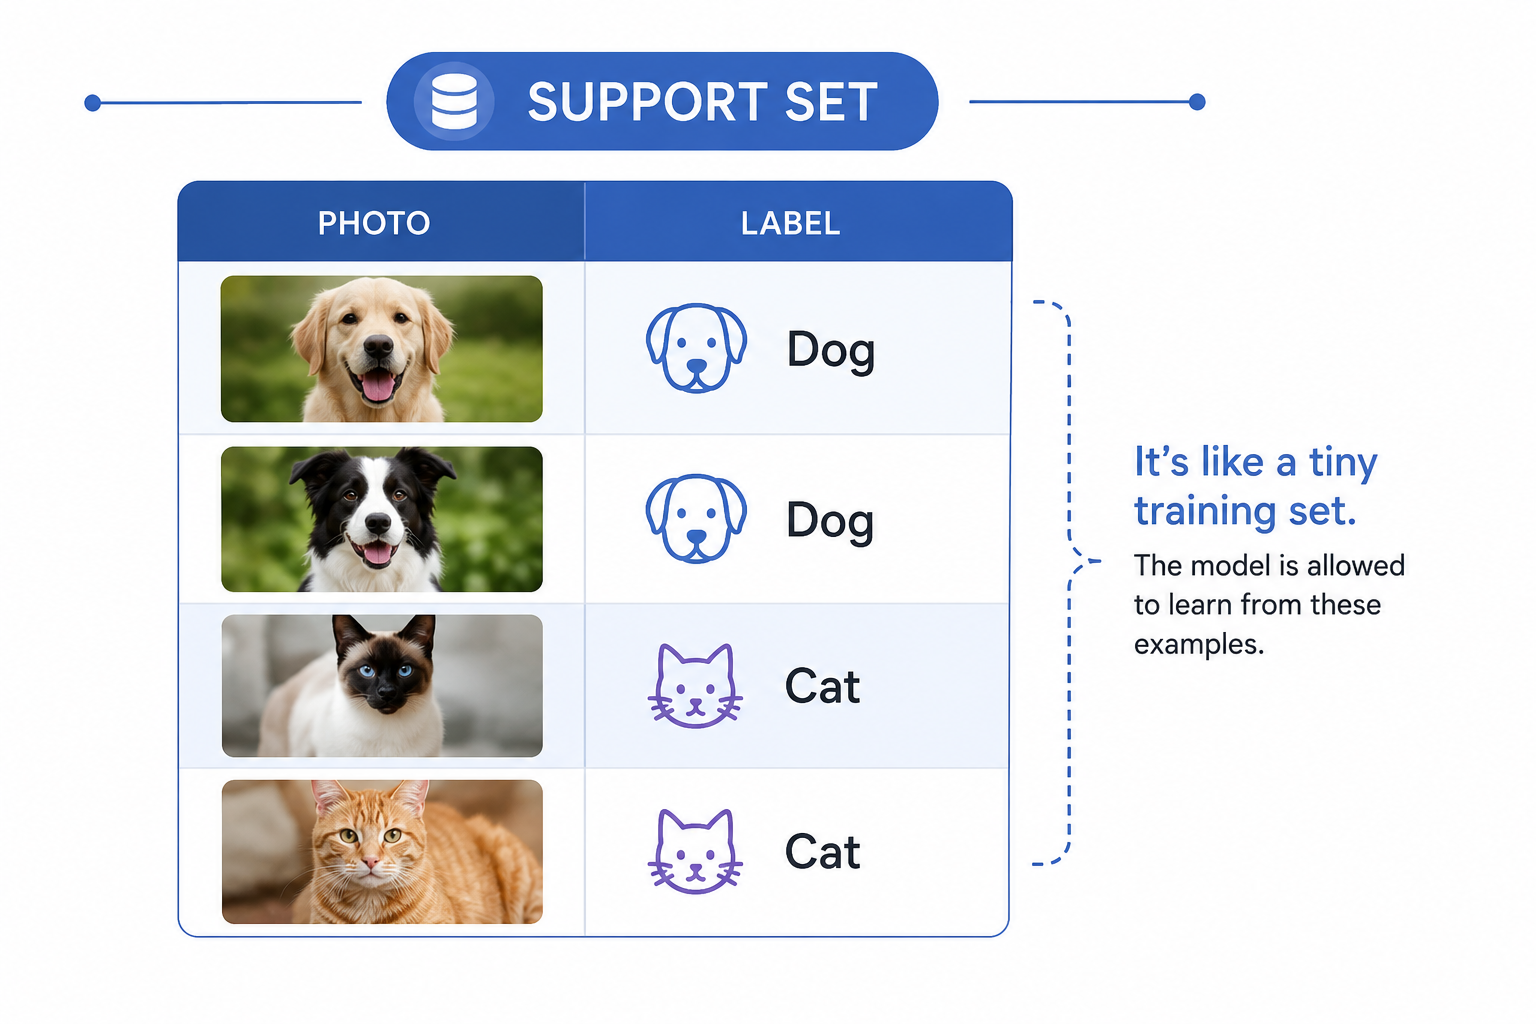
\includegraphics[width=0.85\textwidth]{figures/11-3 figure.png}
\caption{Support Set Structure inside an Episode.}
\label{fig:support_set}
\end{figure}

\textbf{Query Set}:
After studying the Support Set, the model is tested on the Query Set. The model must predict the labels using only what it learned from the Support Set. It is like a tiny test set.

\begin{figure}[H]
\centering
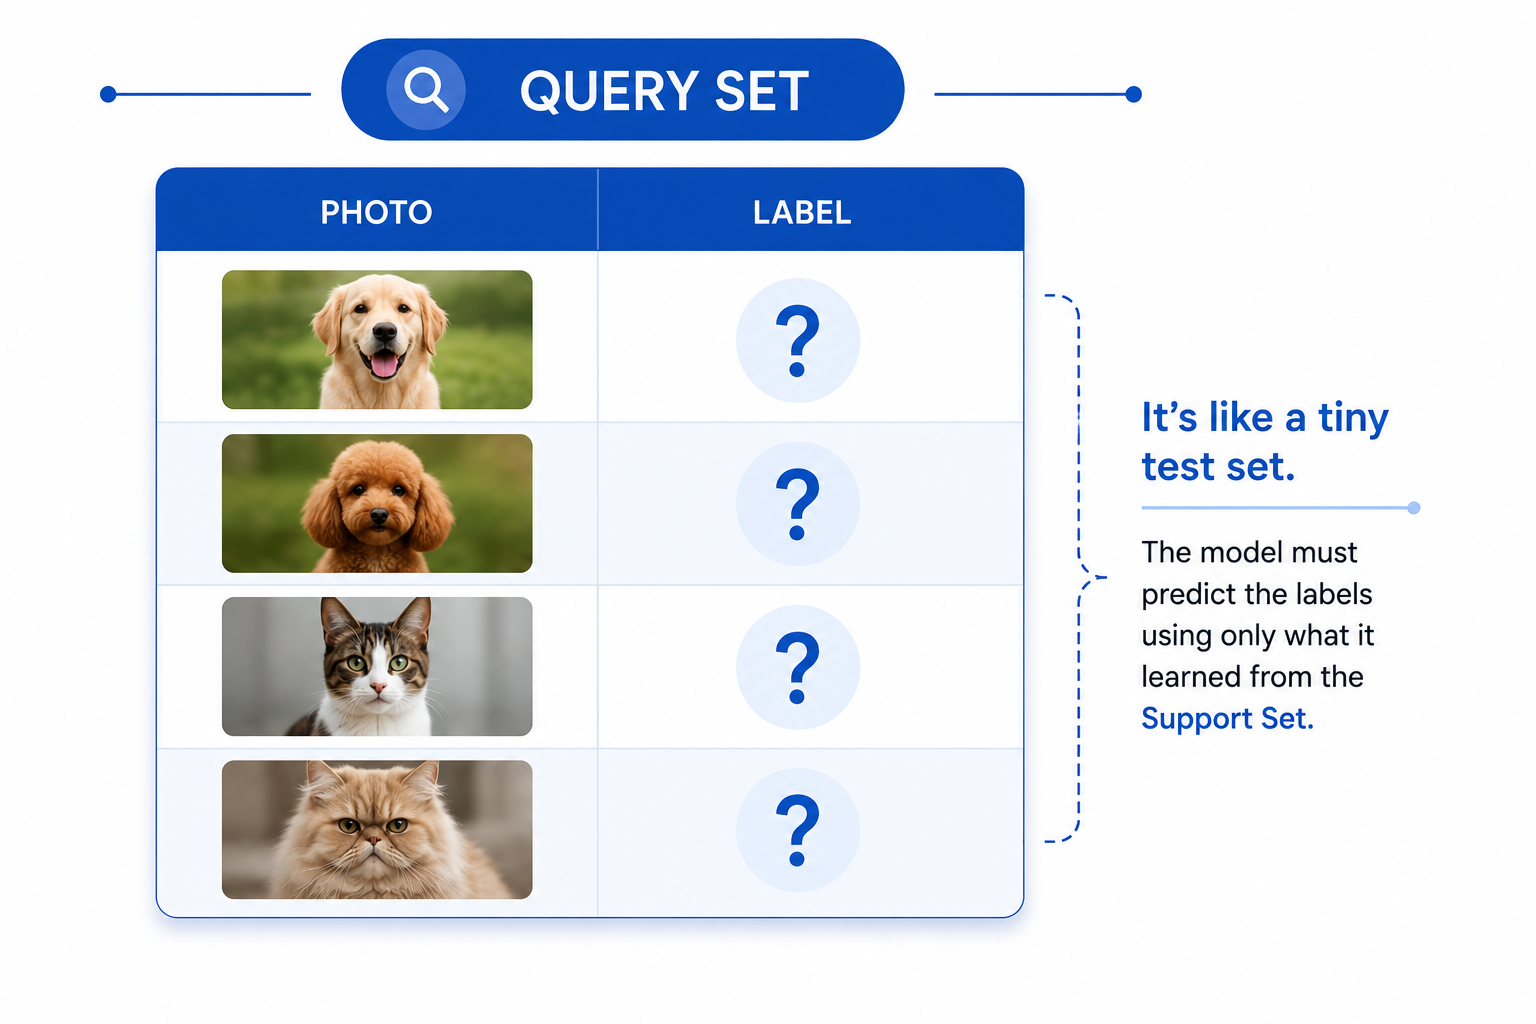
\includegraphics[width=0.85\textwidth]{figures/11-4 figure.png}
\caption{Query Set Structure inside an Episode.}
\label{fig:query_set}
\end{figure}

\subsubsection*{Complete Episode}

A complete episode consists of:
\begin{figure}[H]
\centering
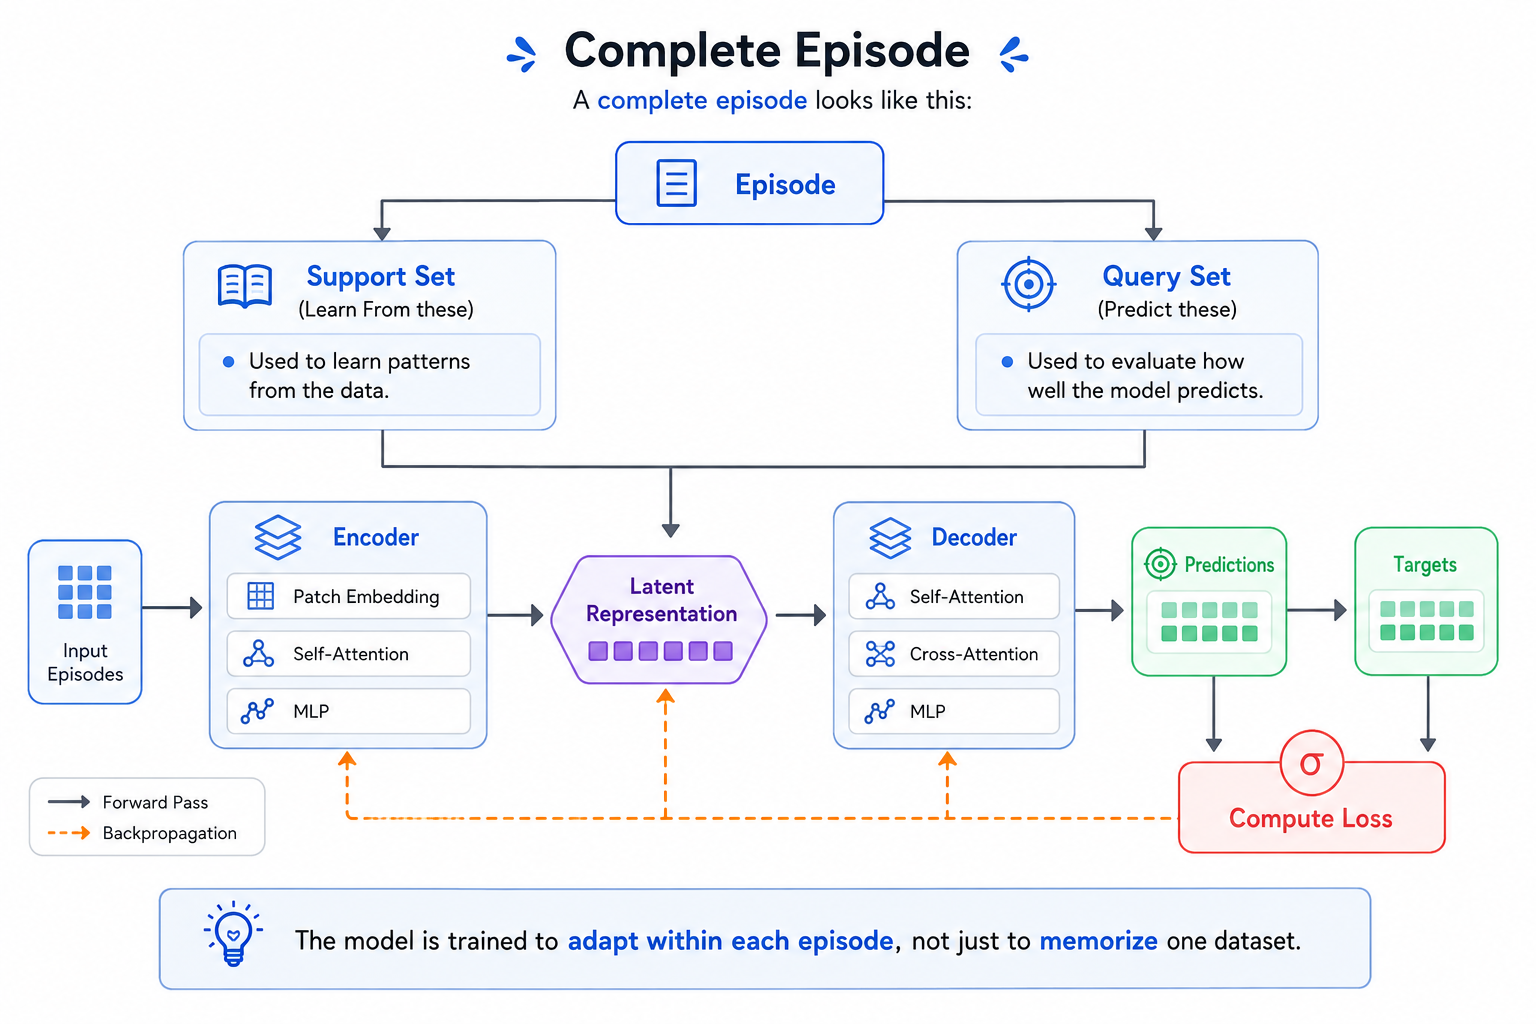
\includegraphics[width=0.95\textwidth]{figures/11-5 figure.png}
\caption{Complete Episode Flow.}
\label{fig:complete_episode}
\end{figure}

The model is trained to adapt within each episode, not just to memorize one dataset.

\subsection*{Meta-Learning Summary}

Meta-Learning addresses the limitation of traditional deep learning, which typically requires large labeled datasets for every new task. Instead of learning a single task, a meta-learning model is trained across many tasks, allowing it to ``Learn to Learn''.

Training is based on episodes, where each episode contains a Support Set (for learning) and a Query Set (for evaluation). This prepares the model to solve new tasks with only a few examples, making it particularly effective for Few-Shot Learning.

\section{Metric-Based Meta-Learning}

\subsection*{1) Siamese Networks}

Traditional Classifiers learn to predict fixed classes. However, in One-Shot or Few-Shot Learning, there are few labeled examples to train a reliable classifier.

Instead of learning ``what is this class?'', a Siamese Network asks: \textbf{``How similar are two inputs?''}

\textbf{Main Idea}: A Siamese Network consists of two identical sub-networks that share the same parameters. It takes two inputs and predicts whether they belong to the same class or different classes.

\begin{figure}[H]
\centering
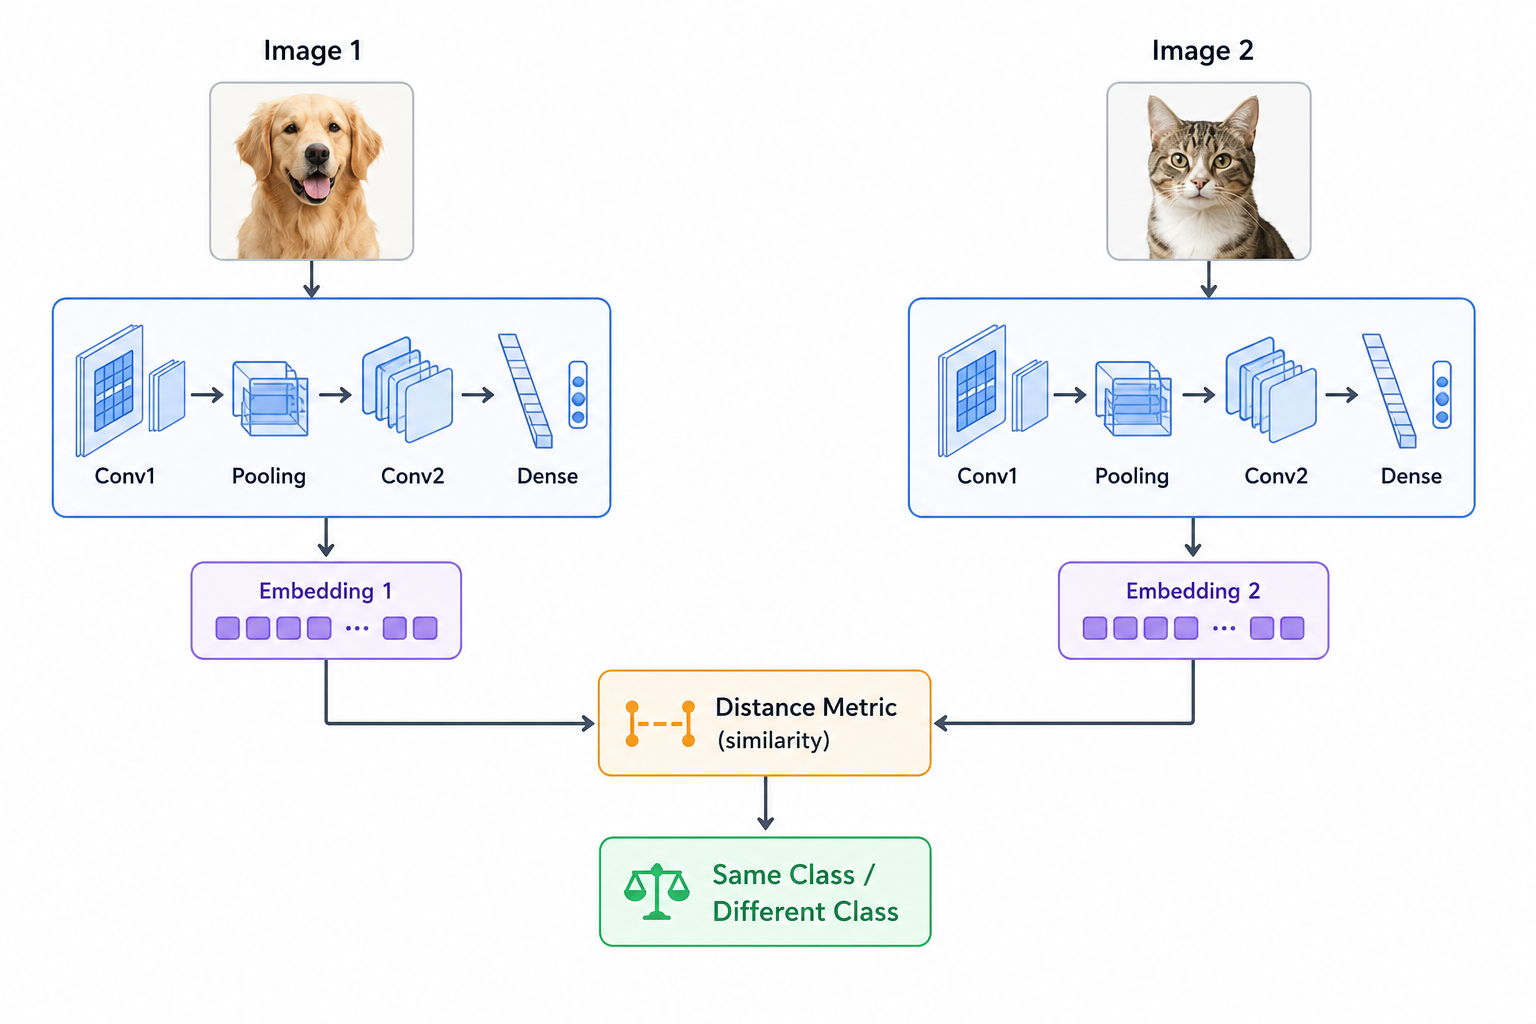
\includegraphics[width=0.95\textwidth]{figures/11-6-1 figure.png}
\caption{Siamese Network Architecture.}
\label{fig:siamese_network}
\end{figure}

The twin networks share the same weights so that both inputs are mapped into the same embedding space and their features are directly comparable.

Siamese Networks are typically trained with Contrastive Loss to pull positive pairs (same class) closer together and push negative pairs (different classes) farther apart.

\textbf{One-Shot Classification}:
When a query image has never been seen before and we only have one support image per class, the query is passed into the Siamese Network with each support image. If the distance is small, the model predicts that class. No retraining needed.

\textbf{Advantages}:
\begin{itemize}
    \item Works with very few examples per class.
    \item No need to retrain the classifier for new classes.
\end{itemize}

\textbf{Limitations}:
\begin{itemize}
    \item Compares image pairs, which means evaluation grows pairwise with many support examples.
    \item Does not create a representative prototype for each class.
\end{itemize}

\subsection*{2) Matching Networks}

In Siamese Networks, classification is performed by comparing individual pairs. Each comparison (Query -- every individual support example) is independent; the model never considers the support set as a whole.

Researchers asked: ``Can the prediction depend on all support images simultaneously?'' This led to Matching Networks.

\textbf{Main Idea}: A query and all support images are first encoded into a common embedding space using a Shared Encoder.

The query embedding is then compared with every support embedding using a similarity measure (Cosine Similarity). The similarities are converted into attention-like weights using Softmax.

The class prediction is obtained as a weighted combination of the support labels, where more similar support examples contribute more to the final prediction.

\begin{figure}[H]
\centering
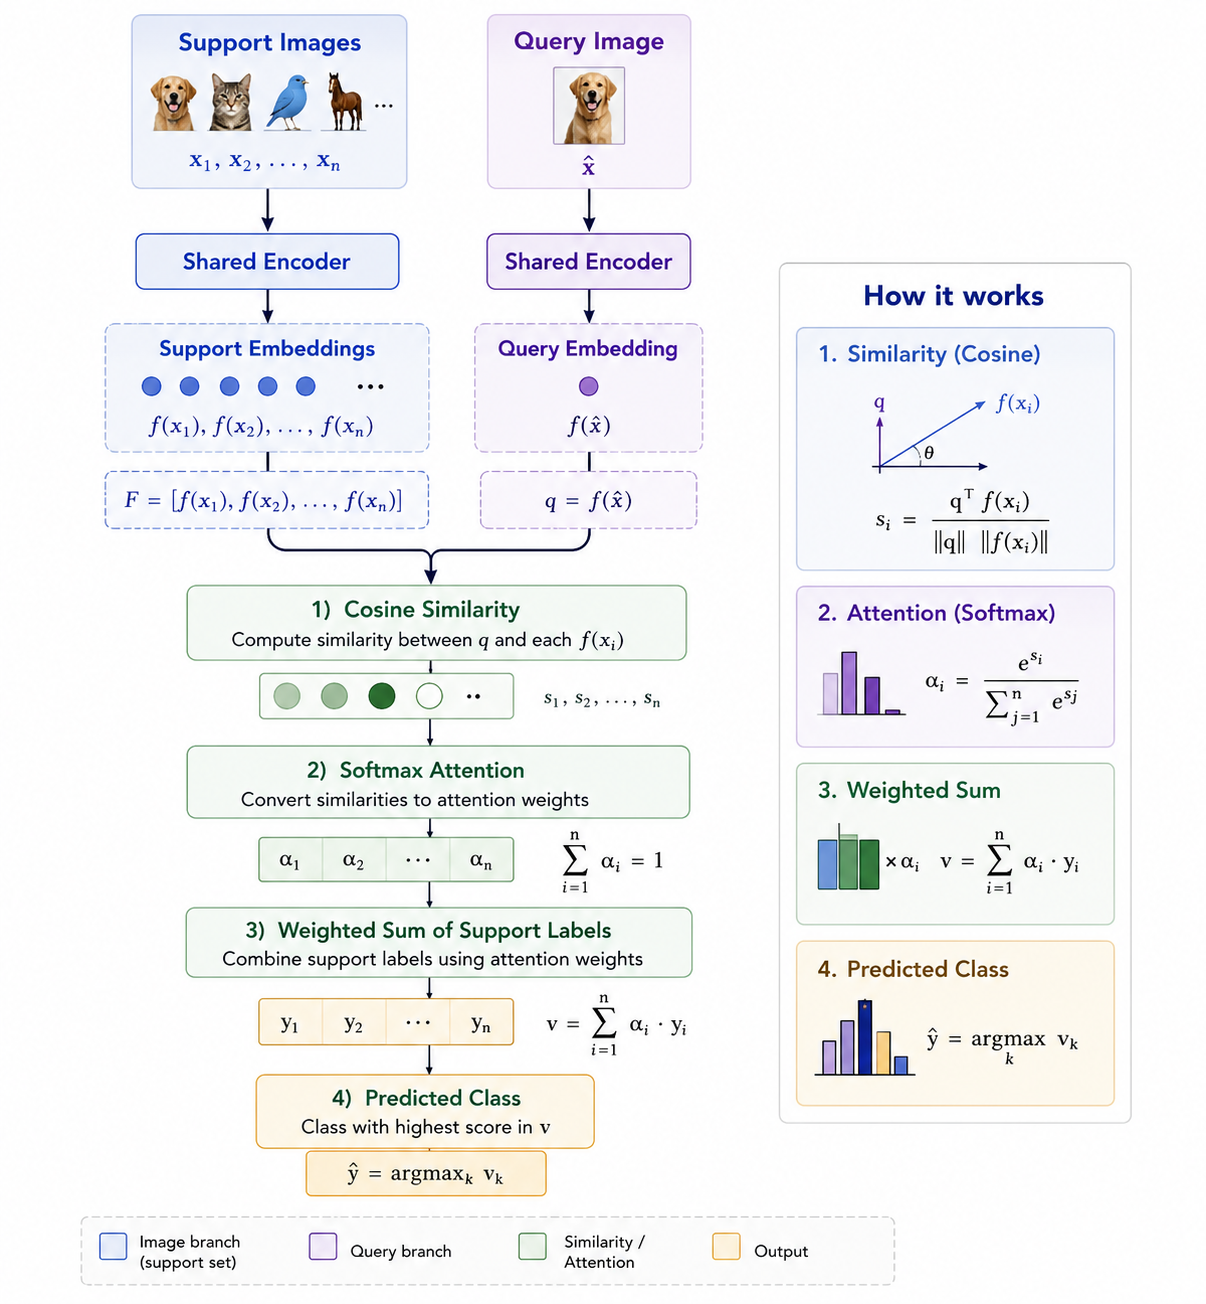
\includegraphics[width=0.95\textwidth]{figures/11-6 figure.png}
\caption{Matching Network Architecture.}
\label{fig:matching_network}
\end{figure}

\textbf{Matching Networks Pipeline}:
\begin{enumerate}
    \item \textbf{Shared Encoder}: Maps both support images and query image to the same embedding space.
    \item \textbf{Cosine Similarity}: Measures similarity between query embedding and each support embedding.
    \item \textbf{Softmax Attention}: Converts similarities to attention weights that sum to 1.
    \item \textbf{Weighted Sum of Labels}: Combines support labels using attention weights.
    \item \textbf{Predicted Class}: Selects the class with the highest score in the weighted sum.
\end{enumerate}

\textbf{Episodic Training}:
Matching Networks introduced an important training strategy: training using episodes, exactly like testing. Each episode contains a Support Set and a Query Set. This teaches the model to solve the same type of few-shot tasks it will encounter during inference.

\textbf{Advantages}:
\begin{itemize}
    \item Uses the entire support set as context instead of isolated pairs.
    \item Naturally handles different support set sizes.
    \item Better few-shot performance than Siamese Networks.
\end{itemize}

\textbf{Limitations}:
\begin{itemize}
    \item Every query must be compared with every support example. When support set size grows, computational cost grows linearly.
    \item Stores individual support embeddings rather than compact class prototypes.
\end{itemize}

\subsection*{3) Prototypical Networks}

In Matching Networks, classifying a query requires comparing it with every support image. If we have 100 support examples per class, the model must compare against 100 images per class.

Researchers asked: ``Do we really need every support example? Or can we store one representation vector per class?''

\textbf{Core Idea}: Instead of storing all support embeddings, Prototypical Networks compute a single Prototype vector for each class by taking the mean embedding of all support examples of that class.

\begin{figure}[H]
\centering
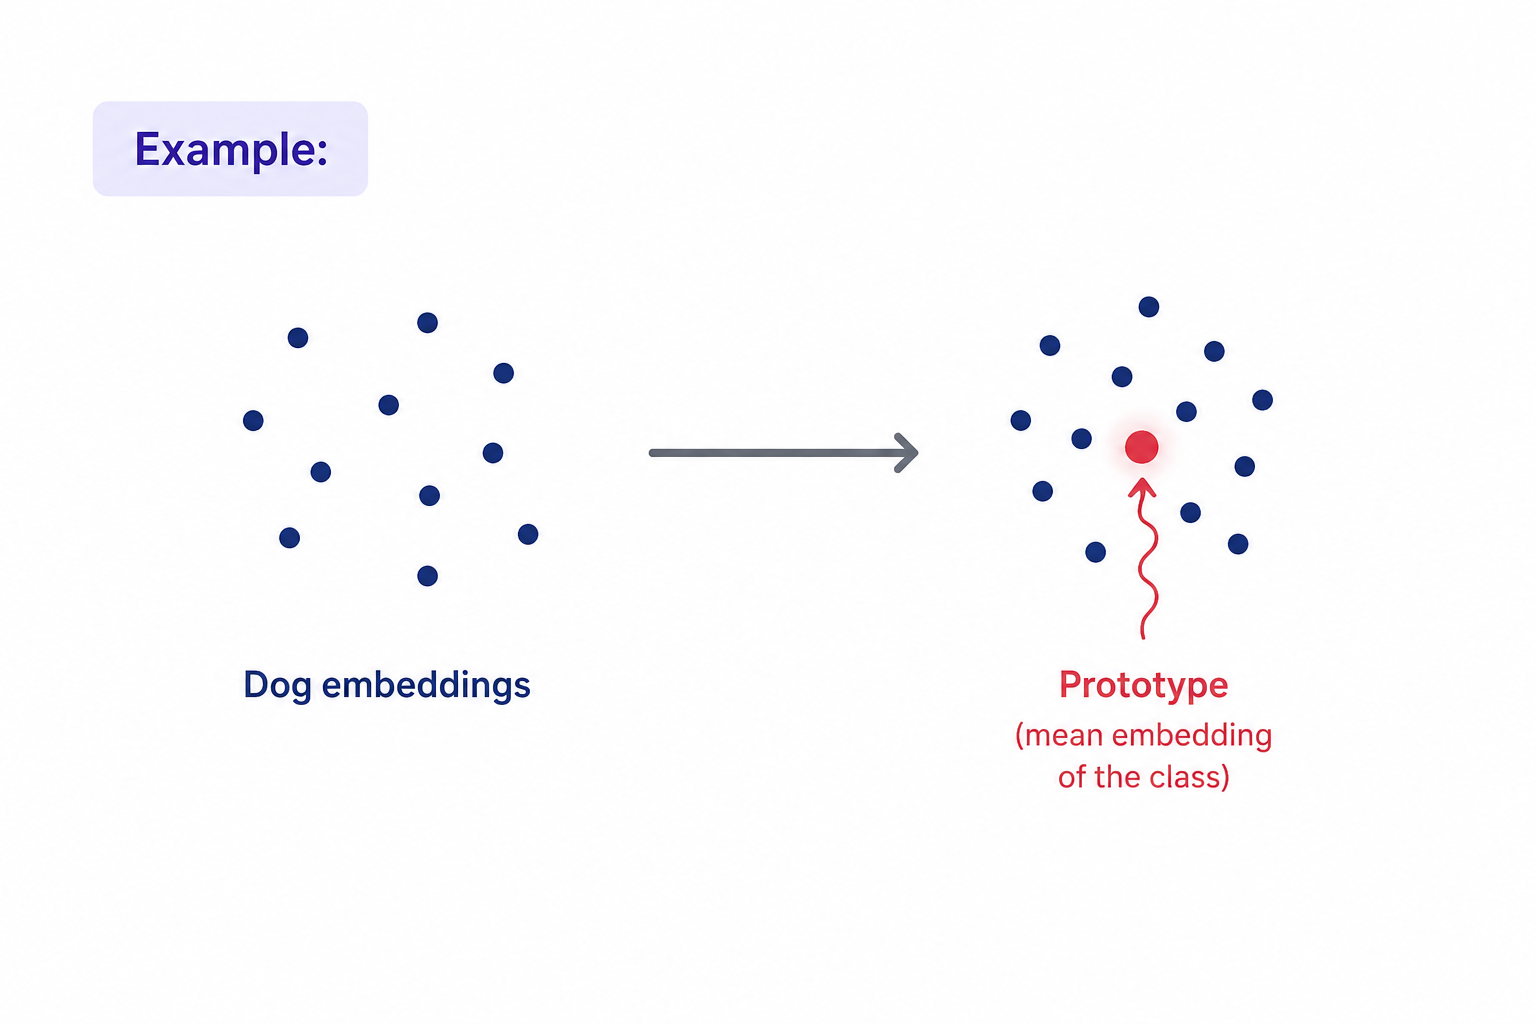
\includegraphics[width=0.85\textwidth]{figures/11-7 figure.png}
\caption{Class Prototypes in Feature Space.}
\label{fig:prototypes_concept}
\end{figure}

Now, every class is represented by one vector (Prototype).

\textbf{Architecture}
\begin{figure}[H]
\centering
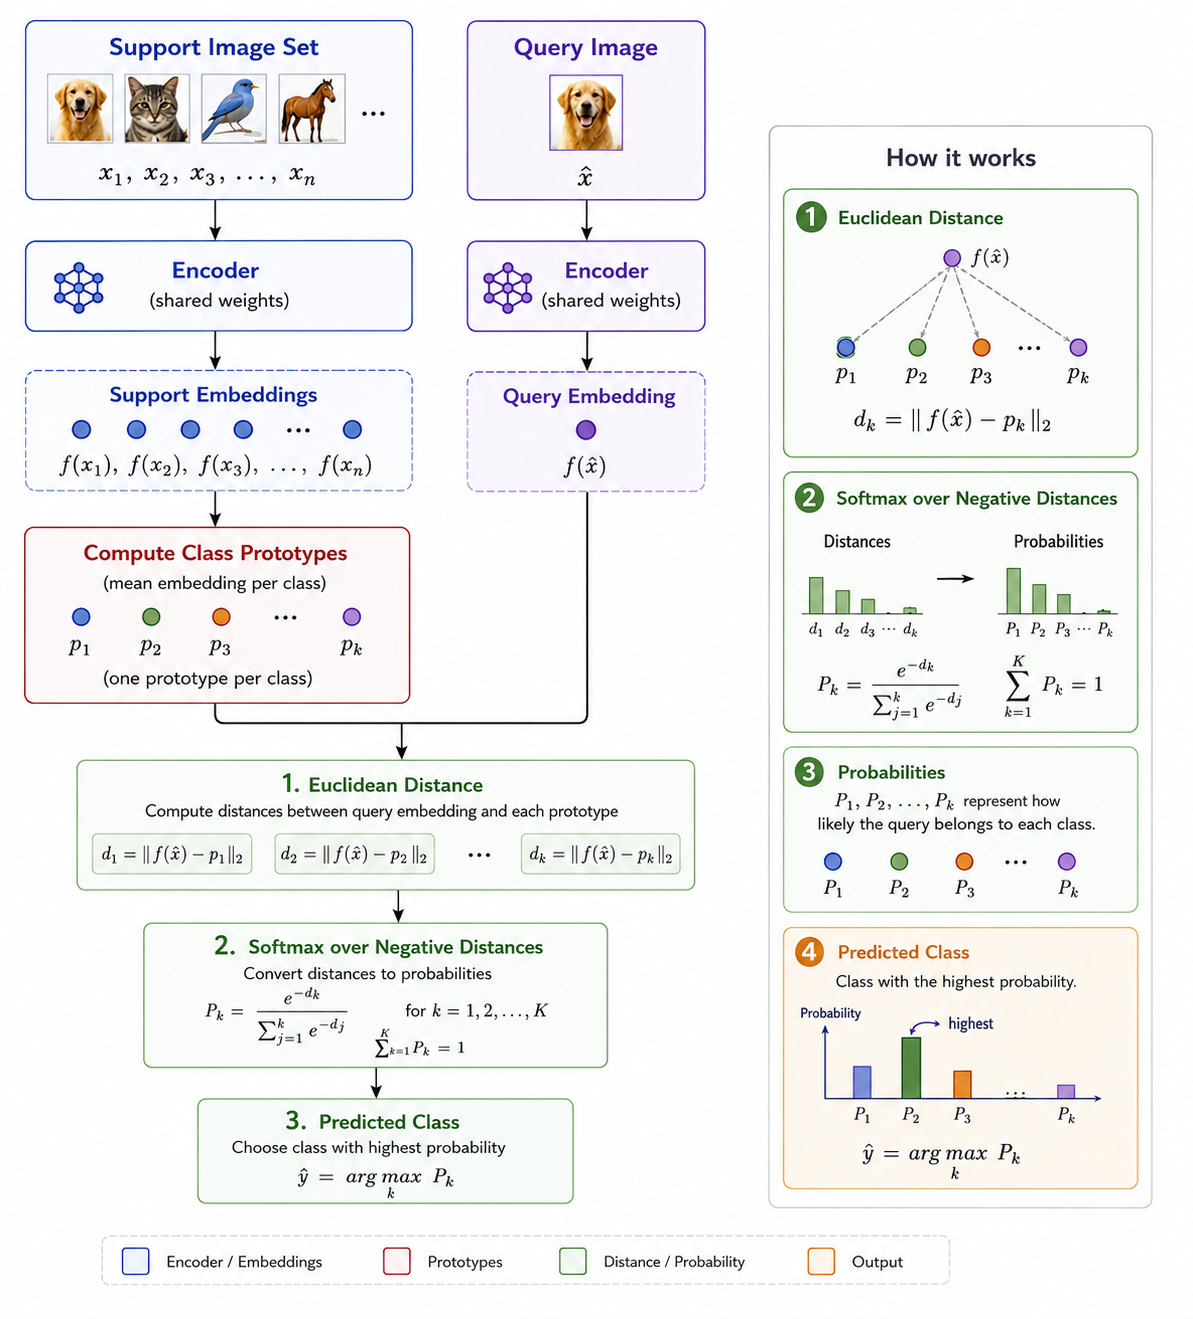
\includegraphics[width=0.80\textwidth]{figures/11-8 figure.png}
\caption{Computation of a Class Prototype as Mean Embedding.}
\label{fig:prototype_mean_embedding}
\end{figure}

During training, the encoder learns an embedding space where:
\begin{itemize}
    \item Samples belonging to the same class cluster together.
    \item Samples from different classes are naturally separated.
\end{itemize}

\begin{figure}[H]
\centering
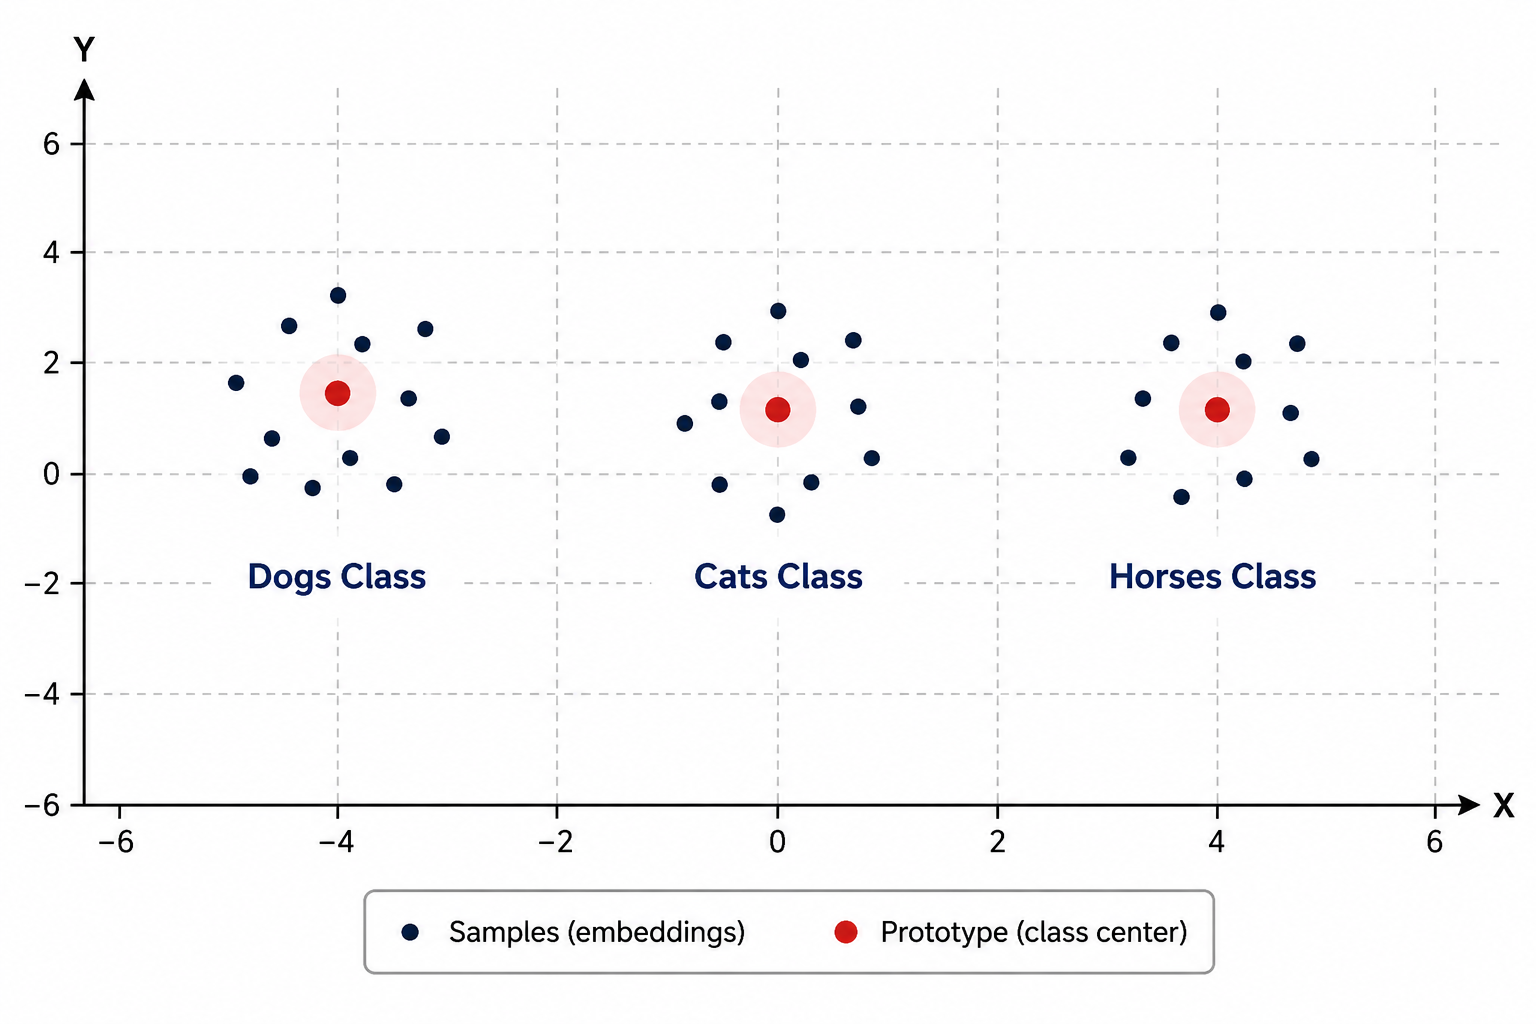
\includegraphics[width=0.95\textwidth]{figures/11-9 figure.png}
\label{fig:prototypical_networks}
\end{figure}

If the embedding space is well learned, the Prototype becomes an excellent representative of its class.

\textbf{How it works}:
\begin{enumerate}
    \item \textbf{Compute Prototypes}: $p_k = \frac{1}{|S_k|} \sum_{x_i \in S_k} f(x_i)$.
    \item \textbf{Euclidean Distance}: Compute distance $d_k = \|f(\hat{x}) - p_k\|^2$.
    \item \textbf{Softmax over Distances}: $P(y = k \mid \hat{x}) = \frac{\exp(-d_k)}{\sum_{k'} \exp(-d_{k'})}$.
    \item \textbf{Predicted Class}: $\hat{y} = \text{argmax}_k P(y = k \mid \hat{x})$.
\end{enumerate}

The encoder learns an embedding space where samples of the same class cluster together and different classes naturally separate.

\textbf{Advantages}:
\begin{itemize}
    \item Simple and fast inference (one comparison per class instead of every image).
    \item Excellent few-shot performance.
\end{itemize}

\textbf{Limitations}:
\begin{itemize}
    \item Assumes each class can be represented by a single center (mean prototype). This assumption fails when classes have complex, multimodal distributions.
\end{itemize}

\begin{figure}[H]
\centering
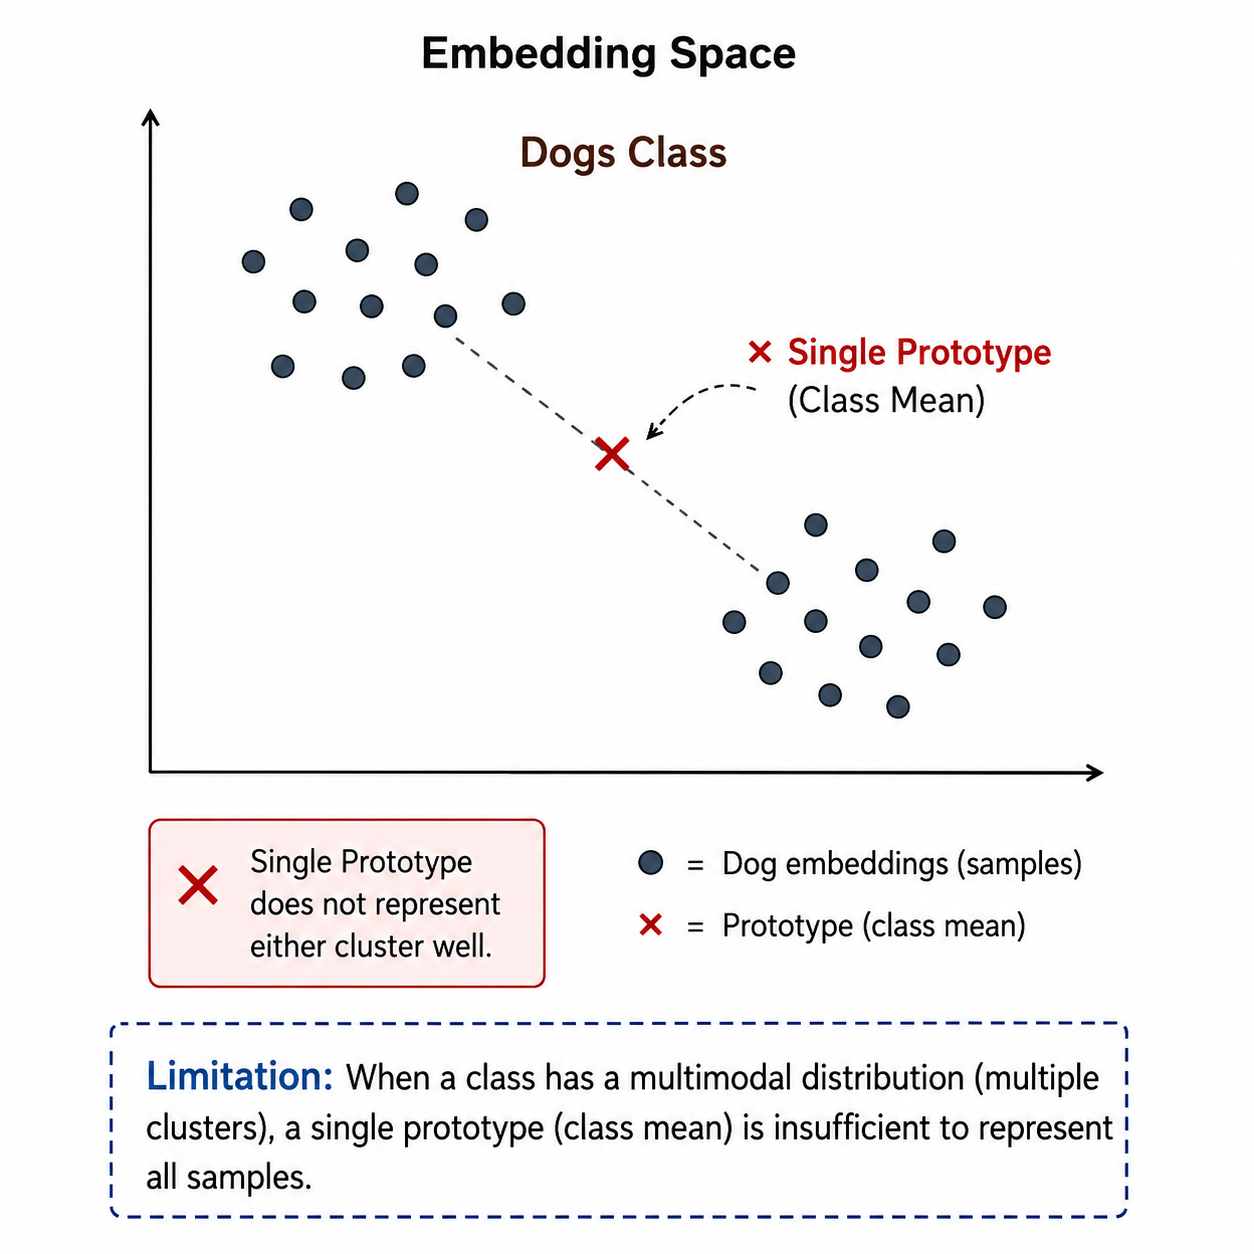
\includegraphics[width=0.95\textwidth]{figures/11-10 figure.png}
\caption{Prototypical Networks Architecture Detail.}
\label{fig:prototypical_networks_detail}
\end{figure}

\subsection*{4) Relation Networks}

In Prototypical Networks, the similarity function is fixed (Euclidean distance).

Researchers asked: ``Why should we manually choose Euclidean or Cosine distance? Can a neural network learn the similarity function itself?''

\textbf{Main Idea}: Relation Networks split the model into two learnable parts:
\begin{enumerate}
    \item \textbf{Embedding Network}: Extracts feature embeddings from images.
    \item \textbf{Relation Network}: A neural network module that outputs a similarity score between 0 and 1 for concatenated support and query feature maps $[s, q]$.
\end{enumerate}

\begin{figure}[H]
\centering
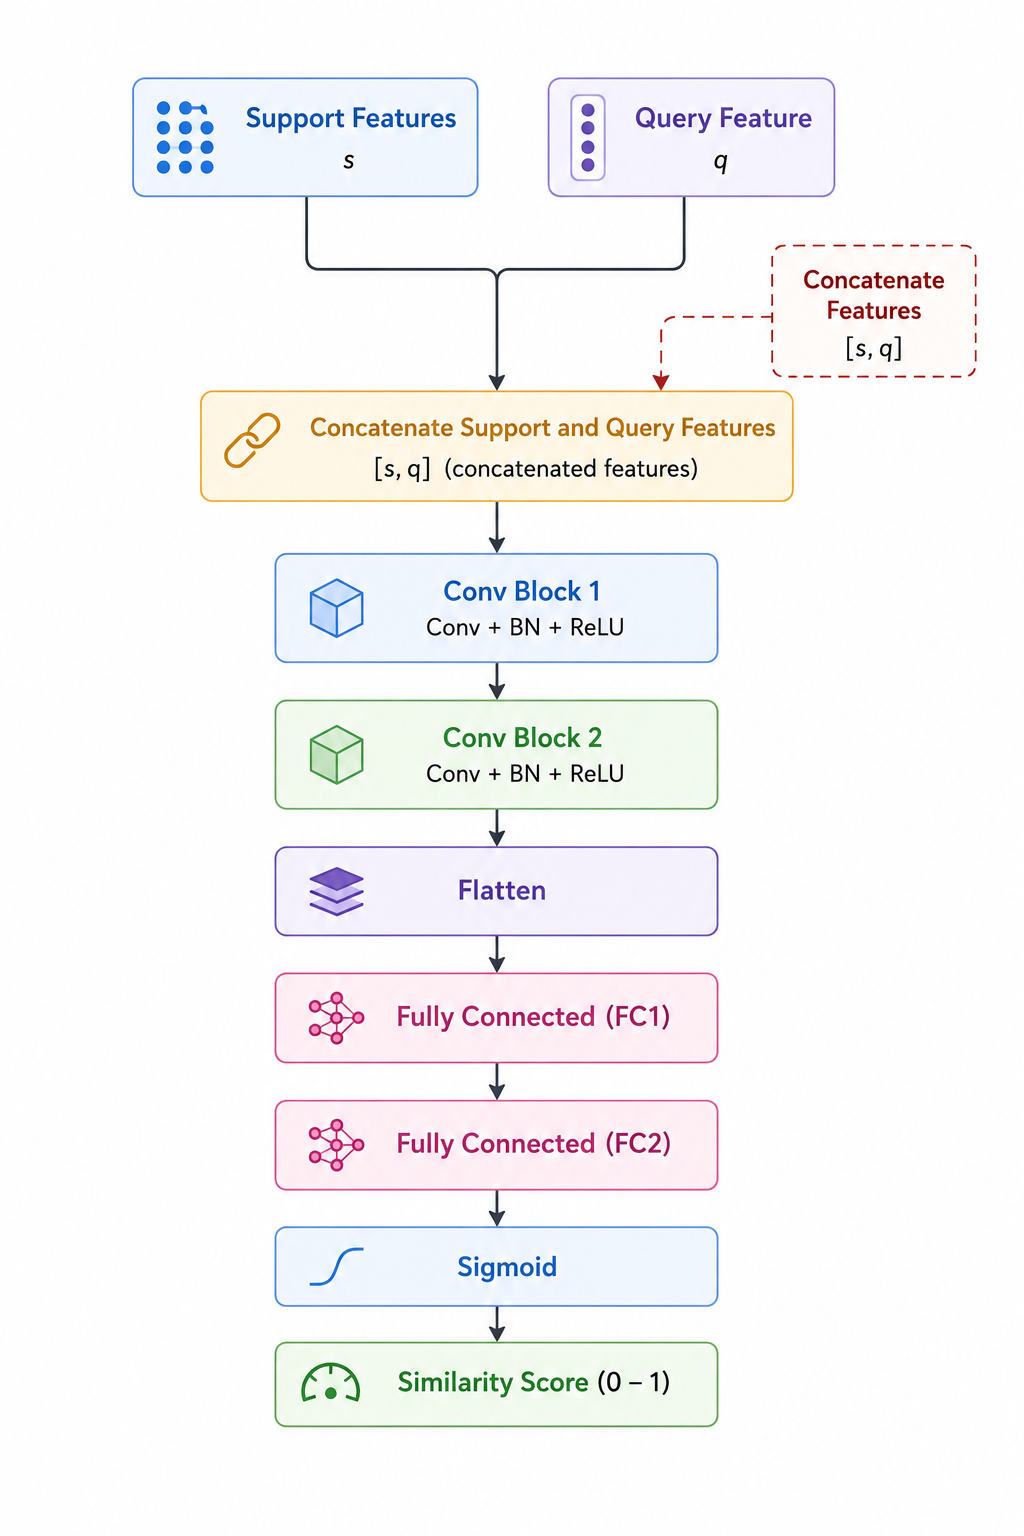
\includegraphics[width=0.95\textwidth]{figures/11-11 figure.png}
\caption{Relation Networks Architecture.}
\label{fig:relation_networks}
\end{figure}

The relation score produced by this network represents how similar the support and query features are.

\begin{figure}[H]
\centering
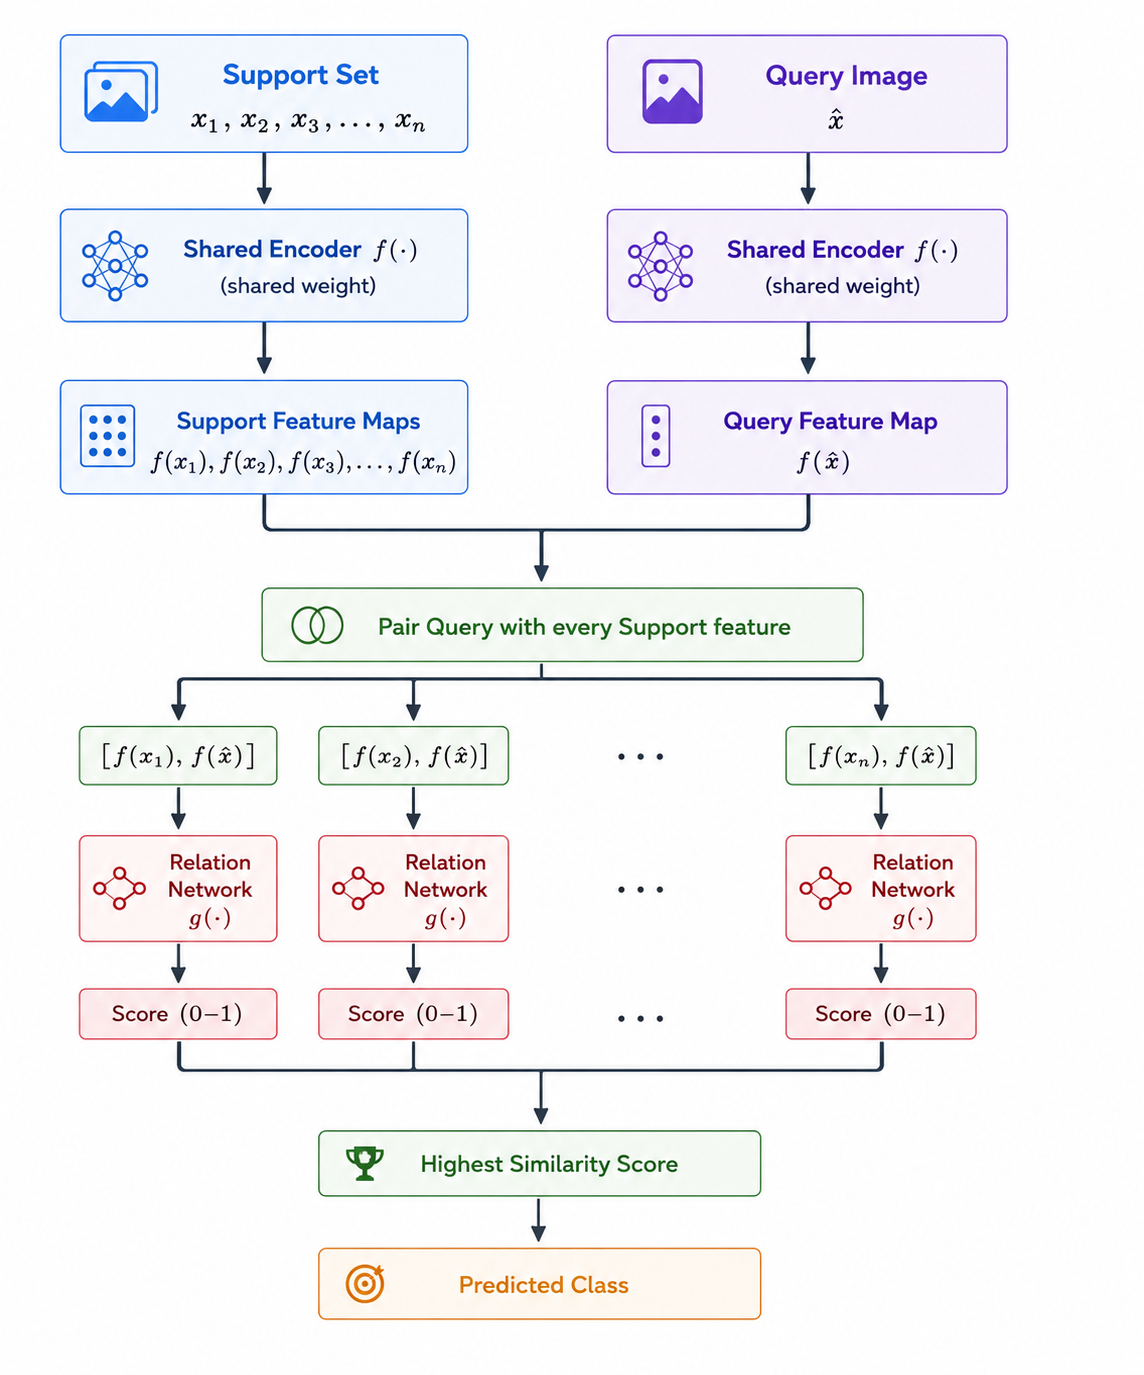
\includegraphics[width=0.75\textwidth]{figures/11-12 figure.png}
\label{fig:relation_module}
\end{figure}

Instead of fixed $\text{Distance}(z_1, z_2)$, we learn $\text{Relation}(z_1, z_2)$ using a Relation Network module.

The Euclidean distance assumes that similarity decreases linearly with distance. However, this assumption is not always valid. Two embeddings may exhibit:

\begin{itemize}
    \item Similar structural patterns.
    \item Correlated features.
    \item Complex nonlinear relationships that cannot be adequately captured by the Euclidean distance.
\end{itemize}

Instead, a learned relation function can automatically discover these underlying patterns and provide a more flexible measure of similarity.

\textbf{Advantages}:
\begin{itemize}
    \item Learns the similarity function instead of relying on a fixed metric.
    \item More flexible than Euclidean distance; can model complex relationships between embeddings.
\end{itemize}

\textbf{Limitations}:
\begin{itemize}
    \item Introduces additional parameters in the relation module.
    \item Higher computational cost and risk of overfitting compared to simple metric-based methods.
\end{itemize}

\section{Optimization-Based Meta-Learning}

\subsection*{Model-Agnostic Meta-Learning (MAML)}

Unlike metric-based methods that learn an embedding space, MAML learns an initial set of model parameters $\theta$ such that, after only a few gradient updates (typically 1--5), the model can rapidly adapt to a new task and achieve high performance.

\begin{figure}[H]
\centering
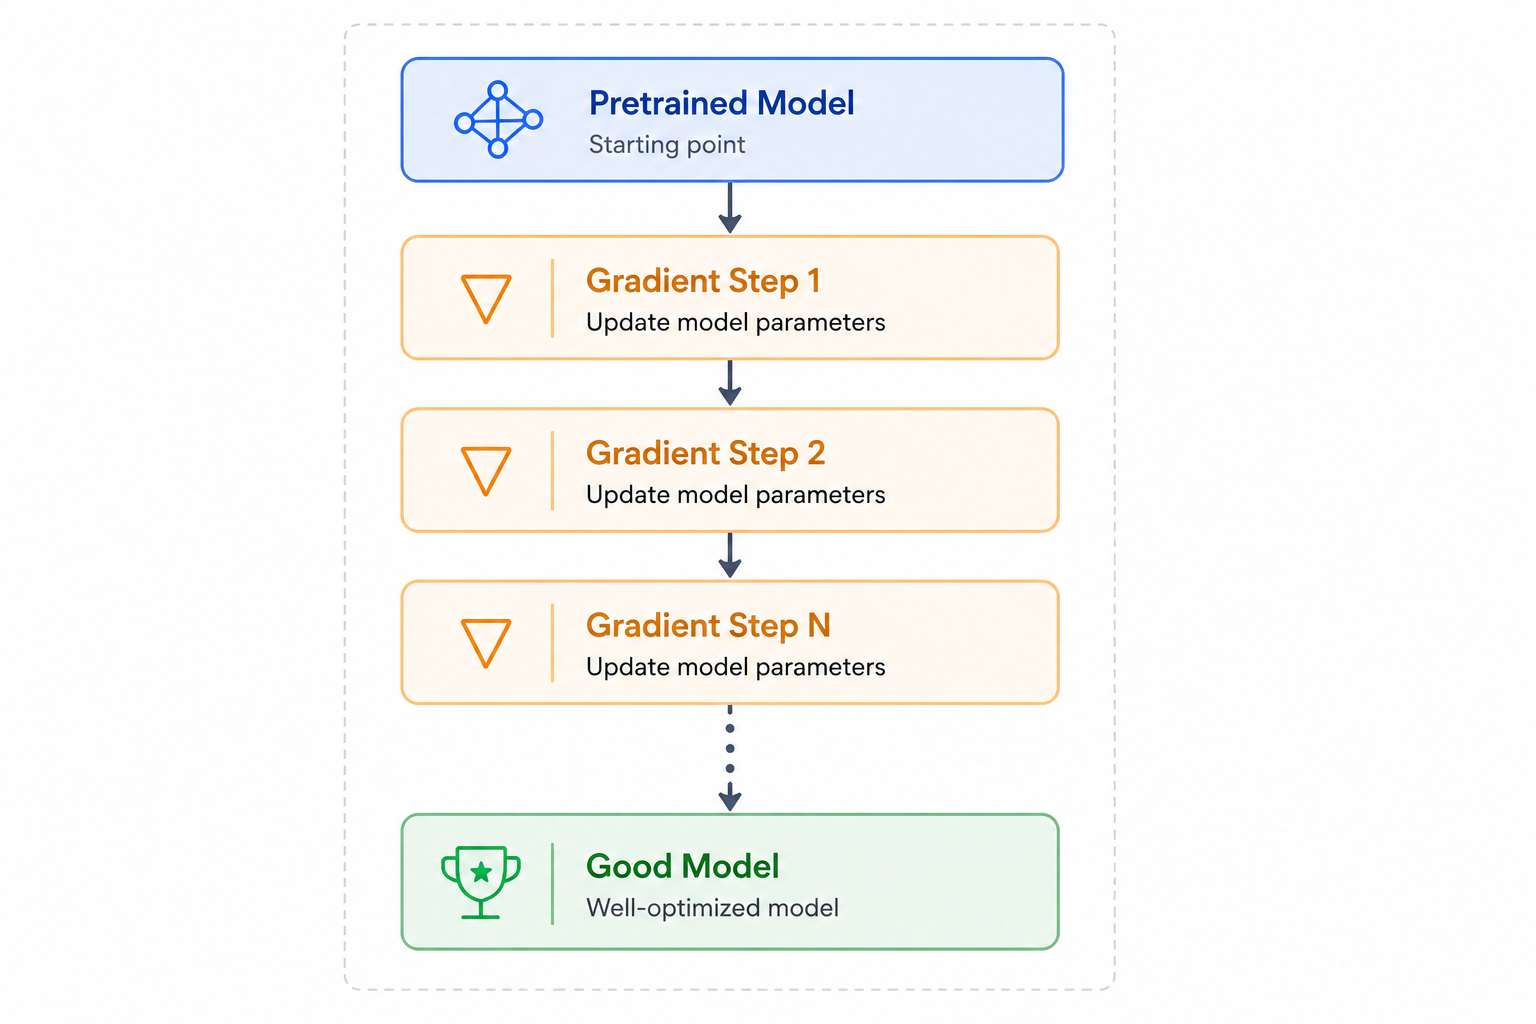
\includegraphics[width=0.65\textwidth]{figures/11-13 figure.png}
\end{figure}

Conventional deep learning models often require hundreds or even thousands of gradient updates to adapt to a new task. In contrast, MAML optimizes the initial parameters so that only a few gradient updates are sufficient for effective adaptation.

\begin{figure}[H]
\centering
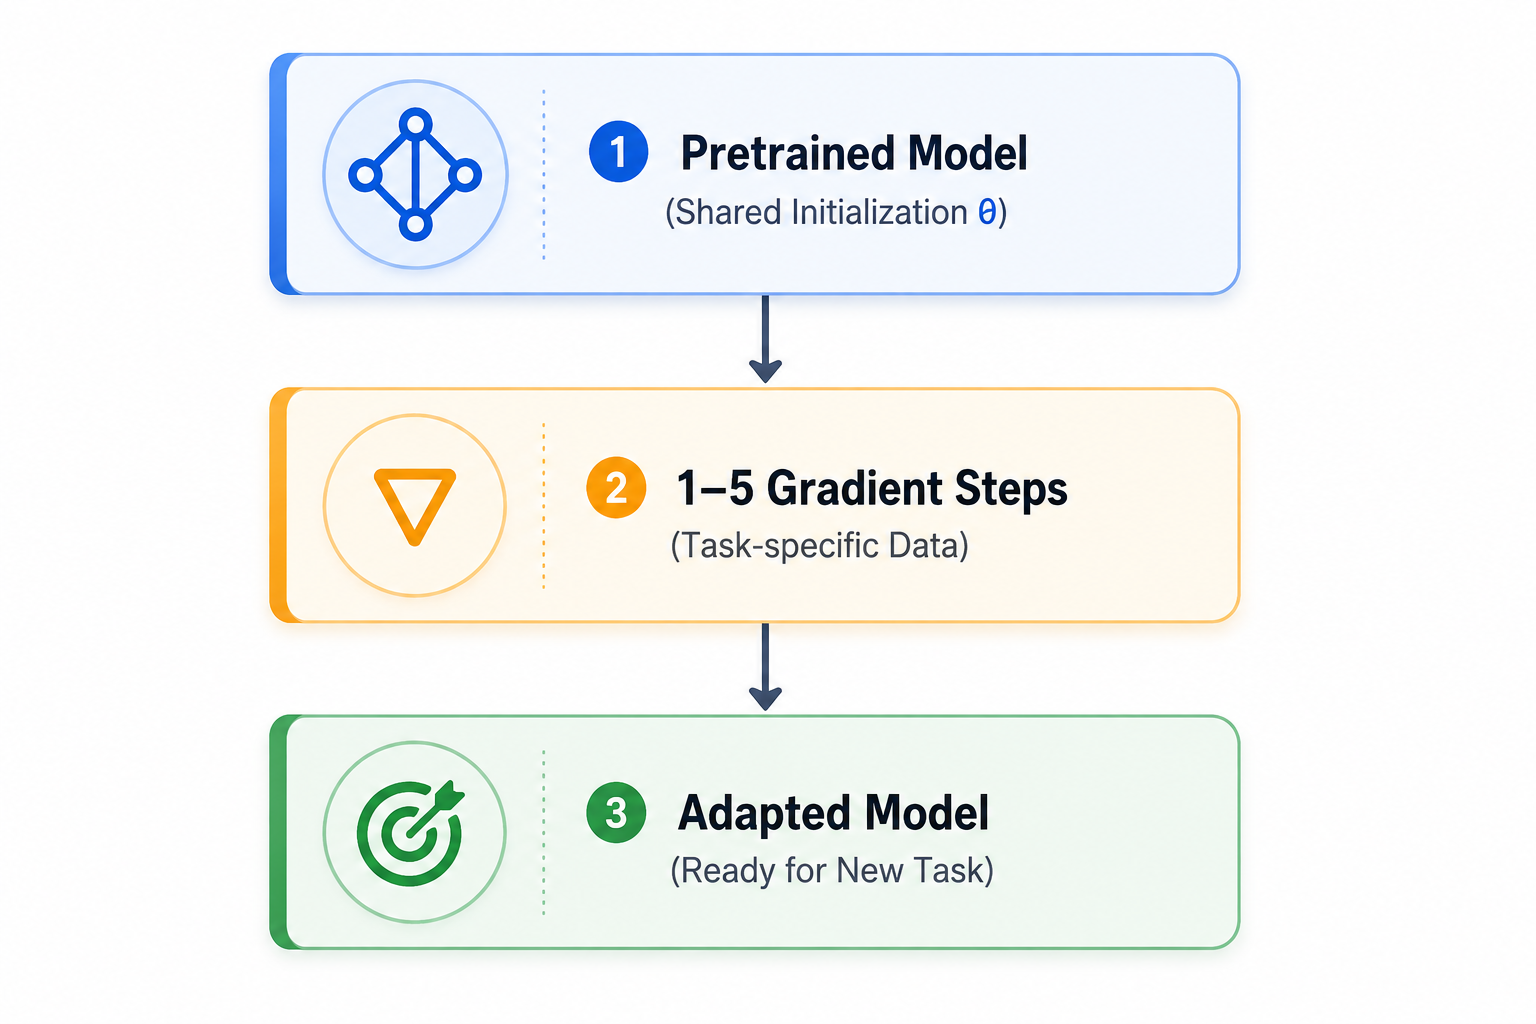
\includegraphics[width=0.65\textwidth]{figures/11-14 figure.png}
\end{figure}

In other words, MAML trains the model to be easy to fine-tune.
\vspace{3cm}
\subsubsection*{Core Idea of MAML}

The goal of MAML is to find an initial parameter vector $\theta$ such that for any new task $\mathcal{T}_i$, the model achieves good performance after taking just $1$--$5$ gradient steps.

Instead of learning a static representation, MAML explicitly optimizes for fast task adaptation.

Like previous meta-learning methods, MAML trains across a set of tasks $\{\mathcal{T}_i\}$ rather than a single dataset.

\begin{figure}[H]
\centering
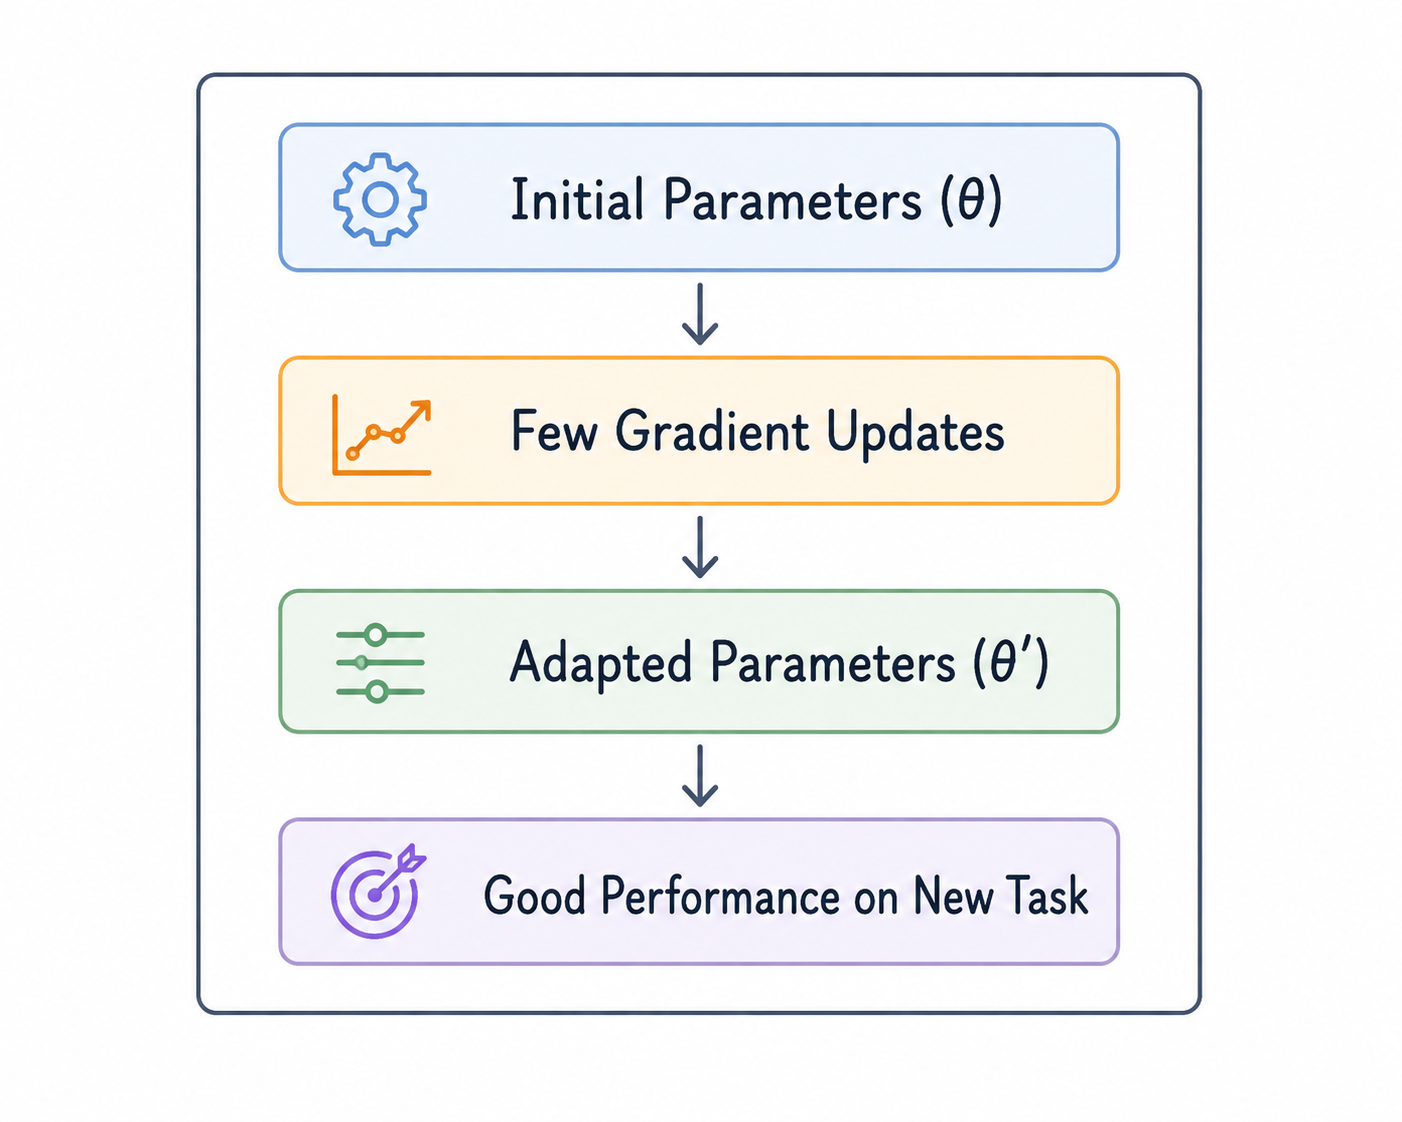
\includegraphics[width=0.95\textwidth]{figures/11-15 figure.png}
\end{figure}

\subsubsection*{The Two Loops of MAML}

MAML operates using two nested optimization loops:

\textbf{1. Inner Loop (Task Adaptation)}:
\begin{itemize}
    \item For each task $\mathcal{T}_i$, the model starts from the current initial parameters $\theta$.
    \item Using the task's Support Set $S_i$, it performs $1$ or a few steps of gradient descent to obtain task-specific parameters $\theta'_i$:
    \[
    \theta'_i = \theta - \alpha \nabla_\theta \mathcal{L}_{\mathcal{T}_i}(\theta)
    \]
    where $\alpha$ is the inner-loop learning rate.
\end{itemize}

\textbf{2. Outer Loop (Meta-Update)}:
\begin{itemize}
    \item The adapted parameters $\theta'_i$ are evaluated on the Query Set $Q_i$ of each task to compute the meta-loss:
    \[
    \mathcal{L}_{\text{meta}}(\theta) = \sum_{\mathcal{T}_i} \mathcal{L}_{\mathcal{T}_i}(\theta'_i)
    \]
    \item The initial parameters $\theta$ are updated using the meta-gradient calculated across all tasks:
    \[
    \theta \leftarrow \theta - \beta \nabla_\theta \sum_{\mathcal{T}_i} \mathcal{L}_{\mathcal{T}_i}(\theta'_i)
    \]
    where $\beta$ is the outer-loop learning rate.
\end{itemize}

\begin{figure}[H]
\centering
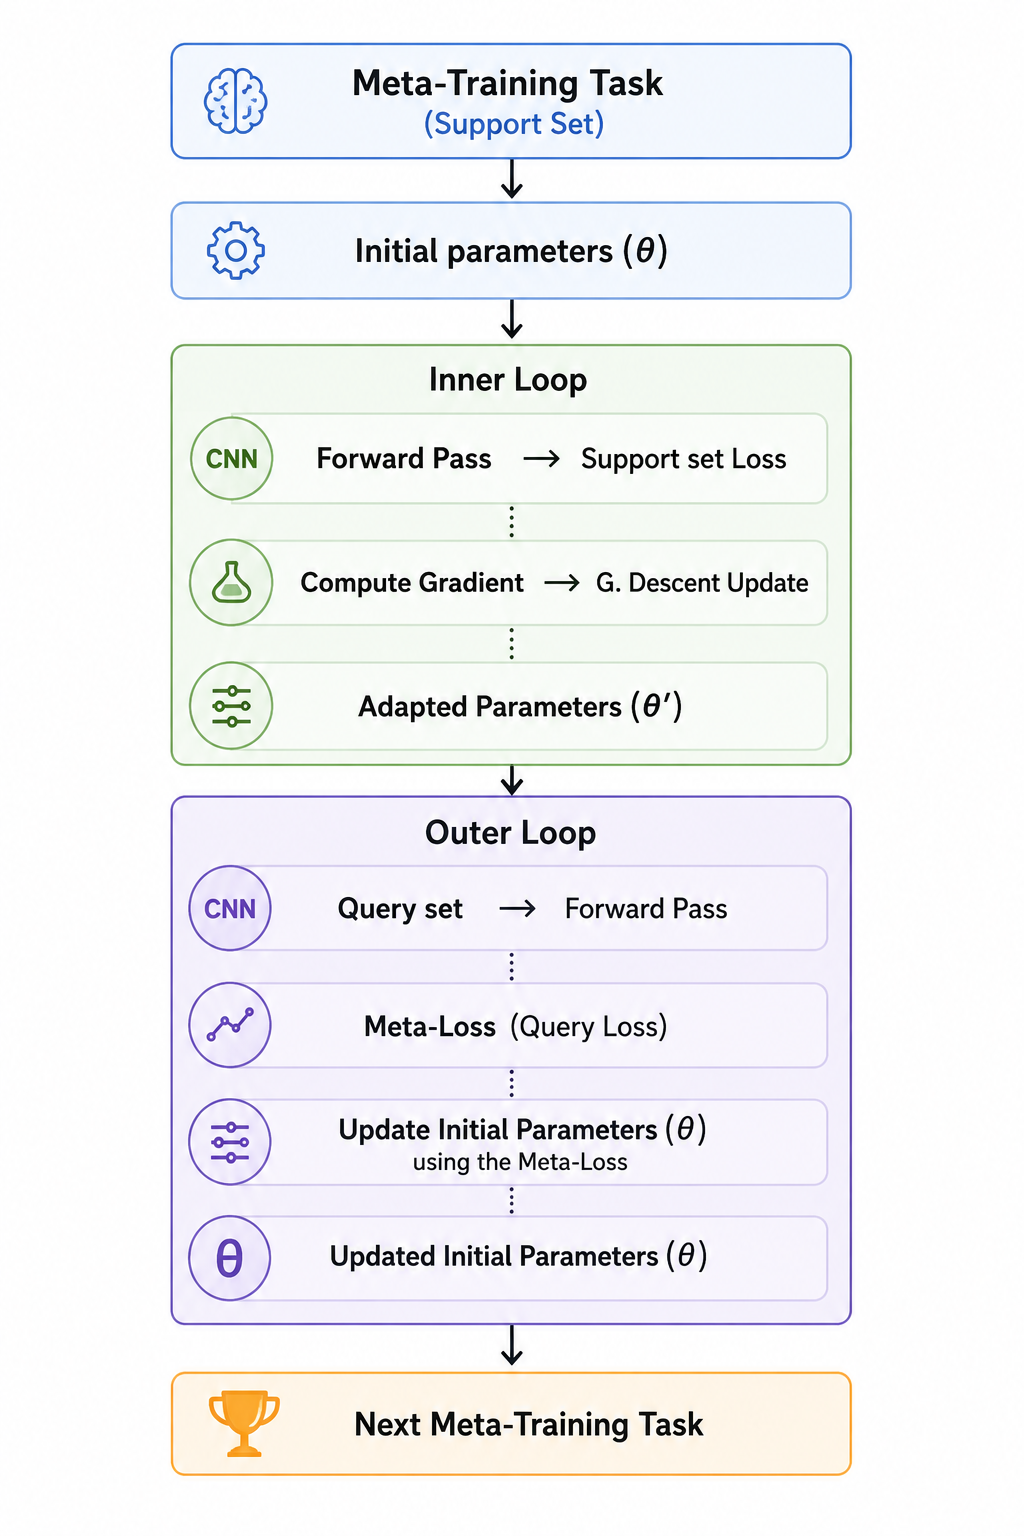
\includegraphics[width=0.95\textwidth]{figures/11-16 figure.png}
\caption{First-Order MAML (FOMAML) Pipeline and Parameter Update Approximation.}
\label{fig:fomaml_pipeline}
\end{figure}

\vspace{0.5cm}
\noindent\rule{\textwidth}{0.4pt}
\vspace{0.5cm}


MAML learns an initial set of parameters $\theta$ that acts as a universal starting point for many different tasks. Instead of optimizing the model for one specific task, MAML optimizes the initialization itself so that the model can adapt to a new task with only a few gradient updates.

\begin{figure}[H]
\centering
\begin{tikzpicture}[
    node distance=1.8cm,
    every node/.style={font=\small},
    block/.style={
        draw,
        rounded corners=5pt,
        thick,
        minimum width=5cm,
        minimum height=1.1cm,
        align=center,
        fill=blue!10
    },
    arrow/.style={
        ->,
        thick,
        >=Stealth
    }
]

\node[block] (random)
{Random Initialization\\$\theta$};

\node[block, below=of random, fill=green!12] (meta)
{Meta-Learned Initialization\\$\theta^\ast$};

\node[block, below=of meta, fill=orange!15] (adapt)
{1--5 Gradient Updates};

\node[block, below=of adapt, fill=purple!12] (task)
{Fast Adaptation to a New Task};

\draw[arrow] (random) -- (meta);
\draw[arrow] (meta) -- (adapt);
\draw[arrow] (adapt) -- (task);

\end{tikzpicture}
\caption{MAML learns a parameter initialization that can rapidly adapt to unseen tasks with only a few gradient updates.}
\end{figure}

After being trained on thousands of different tasks, the learned initialization converges to a region of the parameter space from which most unseen tasks can be solved with only $1$--$5$ gradient updates. Rather than memorizing previous tasks, MAML learns a parameter initialization that enables rapid adaptation to new tasks.
\subsection*{Model-Agnostic Meta-Learning (MAML)}
MAML is model-agnostic, meaning it is not tied to a specific neural network architecture. It can be applied to any model that is trainable using gradient descent. Example: CNN, ResNet, ViT, Transformer, LSTM, MLP.

The only requirement is that the model's parameters can be updated through gradient-based optimization.

This flexibility is the reason behind the name \textbf{Model-Agnostic Meta-Learning (MAML)}.

\subsection*{Advantages and Limitations}

\textbf{Advantages}:
\begin{itemize}
    \item Learns parameters that adapt very quickly.
    \item Works with almost any neural network architecture.
    \item Applicable beyond classification (regression, reinforcement learning...).
\end{itemize}

\textbf{Limitations}:
\begin{enumerate}
    \item \textbf{Computationally Expensive}: Each task requires:
    \begin{itemize}
        \item Forward pass
        \item Backward pass (inner loop)
        \item Another forward/backward pass (outer loop)
    \end{itemize}
    Training is much slower than standard supervised learning.

    \item \textbf{High Memory Usage}: The outer loop needs gradients through the inner optimization steps. This means storing additional computation graphs in memory.

    \item \textbf{Second-Order Derivative}: The original MAML algorithm computes gradients of gradients (second-order derivative). These are mathematically correct but computationally expensive.
\end{enumerate}

This limitation directly motivated the next algorithm: \textbf{First-Order MAML (FOMAML)}.

\section{Why Does MAML Need Second-Order Derivatives?}

For each meta-learning task, MAML performs two optimization stages:
\begin{center}
\begin{tikzpicture}[
every node/.style={font=\small},
block/.style={
draw,
rounded corners=4pt,
minimum width=5.5cm,
minimum height=1cm,
align=center,
thick
},
inner/.style={block,fill=blue!12},
outer/.style={block,fill=green!12},
arrow/.style={->,>=Stealth,thick}
]

% Nodes
\node[inner] (theta)
{$\theta$\\Initial Parameters};

\node[inner, below=1.5cm of theta] (support)
{Support Set\\Compute Loss};

\node[inner, below=1.5cm of support] (update)
{Gradient Update\\$\theta'$};

\node[outer, below=1.5cm of update] (query)
{Query Set\\Compute Loss};

\node[outer, below=1.5cm of query] (meta)
{Meta-Update\\Update $\theta$};

% Arrows
\draw[arrow] (theta) -- (support);
\draw[arrow] (support) -- (update);
\draw[arrow] (update) -- (query);
\draw[arrow] (query) -- (meta);

% Labels
\node[left=2.2cm of support,
font=\bfseries\color{blue},rotate=90]
{Inner Loop};

\node[left=2.2cm of query,
font=\bfseries\color{green!60!black},rotate=90]
{Outer Loop};

\end{tikzpicture}
\end{center}
The objective of the inner loop is to adapt the model to the current task using the Support Set, while the outer loop evaluates the adapted model on the Query Set and updates the initial parameters so that future adaptation becomes faster.
\subsection*{Inner Update}

The adapted parameters are obtained by performing one gradient descent step on the Support Set:

\[
\theta'
=
\theta
-
\alpha
\nabla_{\theta}
\mathcal{L}_{\text{support}}(\theta)
\]

Since the updated parameters $\theta'$ are computed directly from $\theta$, they are not independent. Instead,

\[
\theta' = f(\theta),
\]

which implies

\[
\frac{\partial \theta'}{\partial \theta}\neq0.
\]
\subsection*{Meta-Loss}

After adaptation, the updated model is evaluated on the Query Set:

\[
\mathcal{L}_{\text{meta}}
=
\mathcal{L}_{\text{query}}(\theta').
\]

Although the Meta-Loss is evaluated using $\theta'$, the adapted parameters themselves depend on the original initialization $\theta$. Consequently, the Meta-Loss is also an indirect function of $\theta$.
\subsection*{Backpropagating Through the Inner Update}

To optimize the initial parameters, MAML must differentiate through the gradient update itself.

Using the chain rule,

\[
\boxed{
\frac{\partial \mathcal{L}_{\text{meta}}}{\partial \theta}
=
\frac{\partial \mathcal{L}_{\text{meta}}}{\partial \theta'}
\cdot
\frac{\partial \theta'}{\partial \theta}
}
\]

where

\[
\frac{\partial \theta'}{\partial \theta}
=
I
-
\alpha
\frac{\partial^2
\mathcal{L}_{\text{support}}}
{\partial\theta^2}.
\]

The second derivative (the Hessian) appears because the gradient update itself depends on the gradient of the Support Loss.
\begin{center}
\begin{tikzpicture}[
    every node/.style={font=\small},
    block/.style={
        draw,
        rounded corners=5pt,
        minimum width=5cm,
        minimum height=1cm,
        align=center,
        fill=orange!12,
        thick
    },
    arrow/.style={
        ->,
        >=Stealth,
        thick
    },
    back/.style={
        ->,
        >=Stealth,
        dashed,
        red,
        very thick
    }
]

% Forward pass
\node[block] (theta)
{$\theta$\\Initial Parameters};

\node[block, below=1.4cm of theta] (loss1)
{Support Loss};

\node[block, below=1.4cm of loss1] (grad)
{Gradient Update};

\node[block, below=1.4cm of grad] (theta2)
{Adapted Parameters\\$\theta'$};

\node[block, below=1.4cm of theta2]
(loss2) {Query Loss};

% Forward arrows
\draw[arrow] (theta) -- (loss1);
\draw[arrow] (loss1) -- (grad);
\draw[arrow] (grad) -- (theta2);
\draw[arrow] (theta2) -- (loss2);

% Backward (Meta-Gradient)
\draw[back]
(loss2.west)
to[out=180,in=180]
node[left=0.6cm, align=center]
{\textbf{Meta-Gradient}}
(theta.west);

\end{tikzpicture}
\end{center}
\section{First-Order Model-Agnostic Meta-Learning (FOMAML)}

Although MAML achieves strong few-shot learning performance, its main limitation is the computational cost associated with second-order derivatives. During each meta-update, MAML must backpropagate through the inner optimization step, which requires:

\begin{itemize}
    \item computing second-order derivatives (Hessian-related terms);
    \item storing the complete computation graph for the inner update;
    \item increased GPU memory consumption;
    \item longer training time.
\end{itemize}

To address these limitations, researchers proposed \textbf{First-Order Model-Agnostic Meta-Learning (FOMAML)}, a computationally efficient variant of MAML that removes the need for second-order derivatives while preserving the same meta-learning framework.

The key idea behind FOMAML is that the adapted parameters $\theta'$ are typically very close to the initial parameters $\theta$. Therefore, the dependence of $\theta'$ on $\theta$ is ignored during the computation of the meta-gradient.

\subsection*{First-Order Approximation}

Recall that the exact MAML meta-gradient is

\[
\frac{\partial \mathcal{L}_{\text{meta}}}{\partial \theta}
=
\frac{\partial \mathcal{L}_{\text{meta}}}{\partial \theta'}
\cdot
\frac{\partial \theta'}{\partial \theta}.
\]

FOMAML approximates the Jacobian of the inner update by the identity matrix,

\[
\frac{\partial \theta'}{\partial \theta}
\approx
I,
\]

where $I$ denotes the identity matrix.

Consequently, the meta-gradient simplifies to

\[
\boxed{
\frac{\partial \mathcal{L}_{\text{meta}}}{\partial \theta}
\approx
\frac{\partial \mathcal{L}_{\text{meta}}}{\partial \theta'}
}
\]

This approximation eliminates the computation of Hessian terms, allowing gradients to be computed using only first-order information.

\vspace{0.5cm}

\begin{figure}[H]
\centering
\begin{tikzpicture}[
every node/.style={font=\footnotesize},
block/.style={
draw,
rounded corners=4pt,
minimum width=2.8cm,
minimum height=0.75cm,
align=center,
thick
},
maml/.style={block,fill=blue!12},
fomaml/.style={block,fill=green!12},
arrow/.style={->,>=Stealth,thick},
back1/.style={->,>=Stealth,dashed,red,thick},
back2/.style={->,>=Stealth,dashed,green!60!black,thick}
]

%%%%%%%%%%%%%%%%%%%%%
% MAML
%%%%%%%%%%%%%%%%%%%%%

\node[font=\bfseries] at (-3.5,1.2) {MAML};

\node[maml] (mtheta) at (-3.5,0)
{$\theta$};

\node[maml,below=0.9cm of mtheta] (mupdate)
{Gradient\\Update};

\node[maml,below=0.9cm of mupdate] (mloss)
{Query\\Loss};

\draw[arrow] (mtheta)--(mupdate);
\draw[arrow] (mupdate)--(mloss);

\draw[back1]
(mloss.west)
to[out=180,in=180]
node[left=0.35cm,font=\scriptsize,align=center]
{Second-Order\\Meta-Gradient}
(mtheta.west);

%%%%%%%%%%%%%%%%%%%%%
% FOMAML
%%%%%%%%%%%%%%%%%%%%%

\node[font=\bfseries] at (3.5,1.2) {FOMAML};

\node[fomaml] (ftheta) at (3.5,0)
{$\theta$};

\node[fomaml,below=0.9cm of ftheta] (fupdate)
{Gradient\\Update};

\node[fomaml,below=0.9cm of fupdate] (floss)
{Query\\Loss};

\draw[arrow] (ftheta)--(fupdate);
\draw[arrow] (fupdate)--(floss);

\draw[back2]
(floss.east)
to[out=0,in=0]
node[right=0.35cm,font=\scriptsize,align=center]
{First-Order\\Approximation}
(fupdate.east);

\end{tikzpicture}
\caption{Comparison between MAML and FOMAML. MAML computes second-order meta-gradients by differentiating through the inner update, whereas FOMAML ignores this dependency and uses a first-order approximation.}
\end{figure}



\subsection*{Why Does This Approximation Work?}

During the inner loop, the model performs only a small number of gradient updates (typically 1--5), resulting in relatively small changes to the parameters:

\[
\theta
\longrightarrow
\text{Small Gradient Update}
\longrightarrow
\theta'.
\]

Since $\theta'$ remains close to $\theta$, treating the two parameter sets as approximately equivalent introduces only a small approximation error while substantially reducing computational complexity.

\subsection*{Advantages}

Compared with MAML, FOMAML offers several practical benefits:

\begin{itemize}
    \item significantly lower memory consumption;
    \item faster meta-training;
    \item simpler implementation because no second-order derivatives are required;
    \item performance comparable to MAML on many few-shot learning benchmarks.
\end{itemize}

\subsection*{Limitations}

Despite its computational efficiency, FOMAML remains an approximation of the original MAML algorithm. Consequently,

\begin{itemize}
    \item the computed meta-gradient is not exact;
    \item performance may degrade when the inner-loop updates produce large changes in the model parameters.
\end{itemize}
\section{Reptile}

Although FOMAML eliminates second-order derivatives, it still requires computing a meta-gradient. This raises an important question:

\begin{quote}
\emph{Can meta-learning be achieved without computing a meta-gradient at all?}
\end{quote}

This idea led to \textbf{Reptile}, proposed by OpenAI in 2018.

Reptile is an optimization-based meta-learning algorithm that completely removes the meta-gradient computation. Instead of optimizing the Query Loss as in MAML, Reptile learns a good initialization by repeatedly moving the model parameters toward task-specific solutions obtained after training on individual tasks.

Unlike MAML, Reptile does not explicitly separate each task into a Support Set and a Query Set during the meta-update. Instead, each sampled task is treated as a standard supervised learning problem, and the adapted parameters are used directly to update the initialization.
\subsection*{Training Pipeline}

For each sampled task, Reptile performs the following steps:

\begin{enumerate}
\item Initialize the model with the current parameters $\theta$.
\item Train on the sampled task for a few gradient updates to obtain adapted parameters $\theta'$.
\item Move the initialization slightly toward $\theta'$.
\end{enumerate}
\begin{figure}[H]
\centering
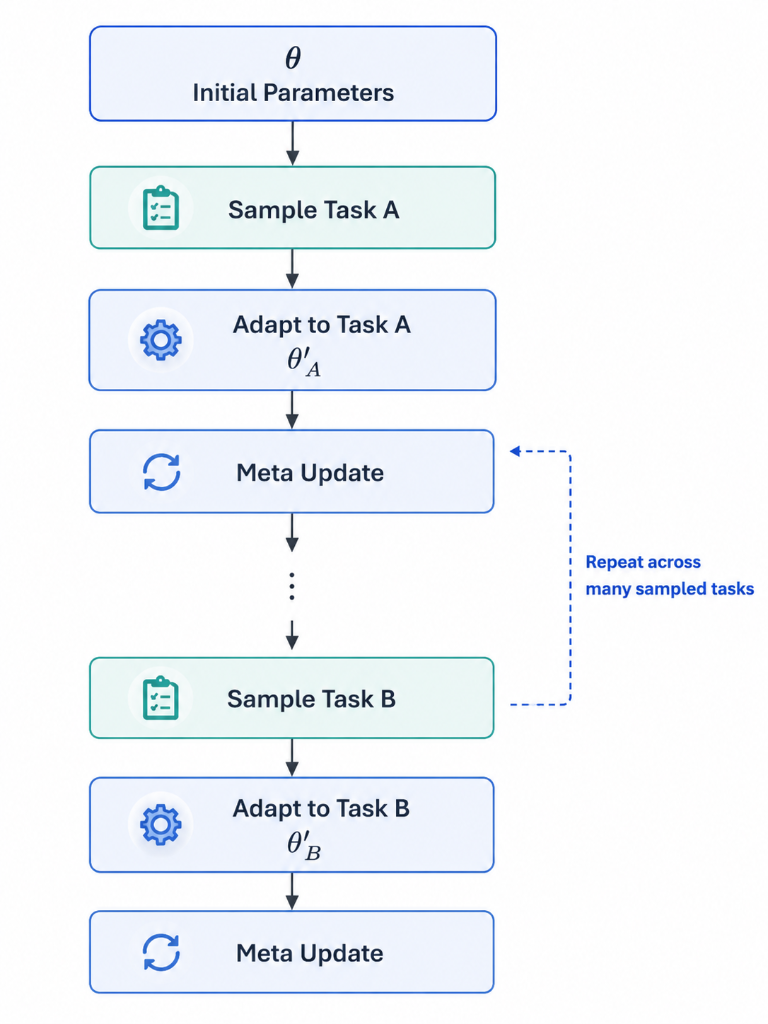
\includegraphics[width=0.55\textwidth]{figures/11-20 figure.png}
\caption{Training procedure of Reptile. For each sampled task, the model is adapted through a few gradient updates to obtain task-specific parameters. The initialization is then updated toward these adapted parameters. Repeating this process across many sampled tasks gradually learns an initialization that can rapidly adapt to unseen tasks.}
\end{figure}




After adapting to a task, Reptile updates the initialization according to

\[
\boxed{
\theta
\leftarrow
\theta
+
\epsilon
(\theta'-\theta)
}
\]

where

\begin{itemize}
\item $\theta$ is the current initialization;
\item $\theta'$ is the adapted parameter vector after training on one task;
\item $\epsilon$ is the meta-learning rate.
\end{itemize}

Rather than replacing the initialization with $\theta'$, Reptile performs only a partial update, gradually moving the initialization toward task-specific solutions.
\subsection*{Meta-Update}

After adapting to a task, Reptile updates the initialization according to

\[
\boxed{
\theta
\leftarrow
\theta
+
\epsilon
(\theta'-\theta)
}
\]

where

\begin{itemize}
\item $\theta$ is the current initialization;
\item $\theta'$ is the adapted parameter vector after training on one task;
\item $\epsilon$ is the meta-learning rate.
\end{itemize}

Rather than replacing the initialization with $\theta'$, Reptile performs only a partial update, gradually moving the initialization toward task-specific solutions.
\subsection*{Why Does Reptile Work?}

Different tasks generally have different optimal parameter values.

\[
\theta
\rightarrow
\theta_A'
\qquad
\theta
\rightarrow
\theta_B'
\qquad
\theta
\rightarrow
\theta_C'
\]

Reptile repeatedly moves the initialization toward the adapted parameters obtained from many different tasks. Over time, the initialization converges to a region of the parameter space that is close to the optima of multiple tasks.

As a result, when a new unseen task is encountered, only a few gradient updates are required to achieve good performance.
\subsection*{Advantages}

Compared with MAML and FOMAML, Reptile offers several practical advantages:

\begin{itemize}
\item no second-order derivatives;
\item no meta-gradient computation;
\item low memory consumption;
\item fast meta-training;
\item simple implementation using any standard optimizer;
\item competitive performance on many few-shot learning benchmarks.
\end{itemize}
\subsection*{Limitations}

Reptile remains an approximation of the meta-learning objective because it never explicitly optimizes the Query Loss. Consequently,

\begin{itemize}
\item it may perform slightly worse than MAML on more challenging tasks;
\item its updates are less theoretically grounded than the exact meta-gradient used by MAML.
\end{itemize}

Nevertheless, the simplicity and computational efficiency of Reptile make it an attractive choice for large-scale few-shot learning problems and resource-constrained environments.

\section{Memory-Based Meta-Learning}

The meta-learning methods presented so far can be broadly divided into two categories:

\begin{itemize}
    \item \textbf{Metric-based methods}, such as Siamese Networks, Matching Networks, Prototypical Networks, and Relation Networks, which perform adaptation by comparing learned feature representations.
    \item \textbf{Optimization-based methods}, such as MAML, FOMAML, and Reptile, which adapt the model parameters through gradient-based optimization.
\end{itemize}

Although these approaches differ in their adaptation mechanisms, they share a common characteristic: the knowledge acquired during training is primarily stored in the model parameters.

Memory-Based Meta-Learning introduces a different paradigm by equipping the model with an \textbf{external differentiable memory}. Instead of encoding all task-specific knowledge in the network weights, the model dynamically stores and retrieves information from this external memory during inference. Consequently, adaptation is achieved by updating the memory contents rather than modifying the model parameters.

One of the earliest and most influential architectures following this paradigm is the \textbf{Memory-Augmented Neural Network (MANN)}.
\begin{figure}[H]
\centering
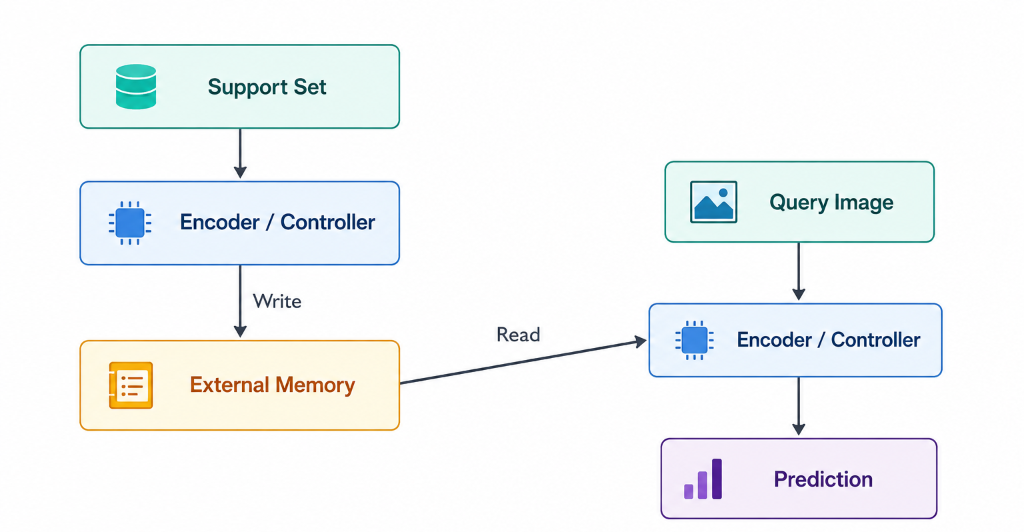
\includegraphics[width=0.85\textwidth]{figures/11-21 figure.png}
\caption{Overview of a Memory-Augmented Neural Network (MANN). Support examples are encoded and written into an external memory. During inference, the query representation retrieves relevant information from memory to produce the final prediction.}
\end{figure}
\subsection*{Architecture}
\begin{figure}[H]
\centering
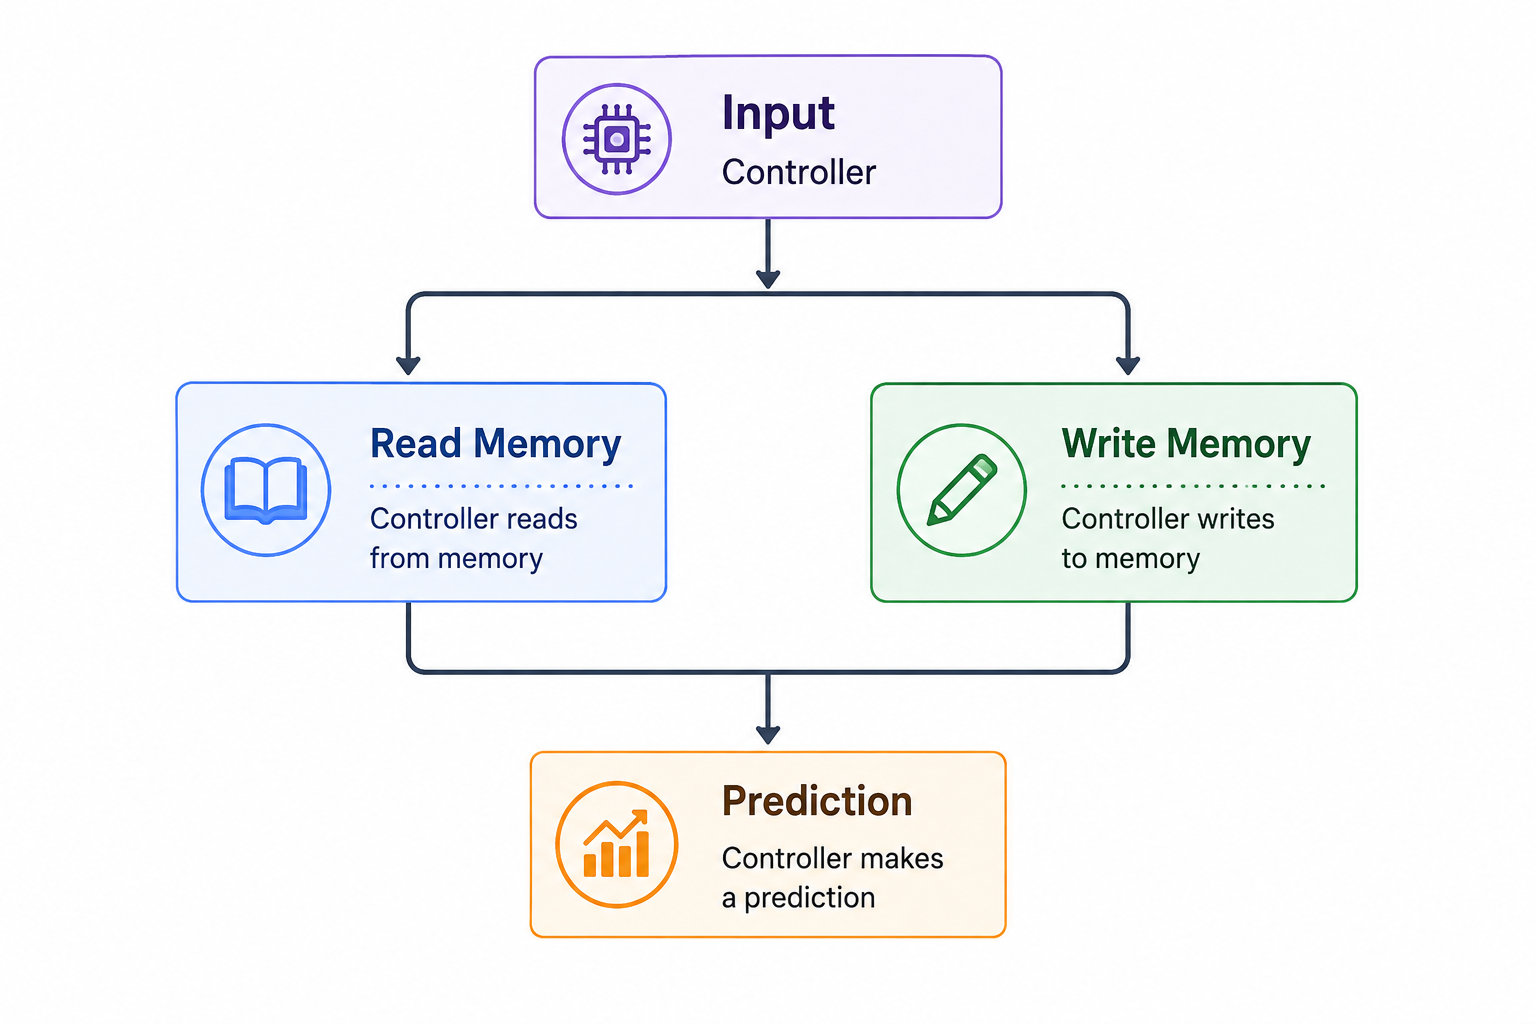
\includegraphics[width=0.95\textwidth]{figures/11-19 figure.png}
\end{figure}

A typical Memory-Augmented Neural Network consists of two main components:

\begin{enumerate}
\item A \textbf{controller}, usually implemented using an LSTM or a Transformer, responsible for interacting with the external memory.
\item An \textbf{external memory}, represented as a differentiable memory matrix that stores task-specific information.
\end{enumerate}
\subsection*{Memory Operations}

During the support phase, each support example is encoded into a feature representation. The controller writes these representations into the external memory, allowing the model to accumulate information about the current task.

During inference, the query image is encoded by the same controller. Rather than relying solely on the network weights, the controller retrieves the most relevant information from the external memory. The retrieved memory is then combined with the query representation to generate the final prediction.
\subsection*{Why Does It Work?}

Unlike optimization-based meta-learning methods, MANNs do not perform gradient updates during inference. Adaptation occurs by dynamically modifying the memory contents while keeping the model parameters fixed. This enables rapid adaptation to unseen tasks without requiring additional optimization.
\subsection*{Advantages}

\begin{itemize}
\item rapid adaptation without gradient updates;
\item dynamic storage of task-specific information;
\item efficient inference for few-shot learning;
\item well suited for sequential and online learning scenarios.
\end{itemize}

\subsection*{Limitations}

\begin{itemize}
\item limited memory capacity;
\item effective performance depends on learning appropriate read and write operations;
\item computational cost increases as the memory size grows.
\end{itemize}
\subsection*{Comparison of Meta-Learning Paradigms}


\begin{table}[H]
\centering
\caption{Comparison of the main meta-learning paradigms.}
\label{tab:meta_learning_comparison}
\renewcommand{\arraystretch}{1.3}

\renewcommand{\arraystretch}{1.35}

\begin{tabularx}{\textwidth}{
>{\bfseries}p{2.8cm}
X
p{2.9cm}
X}
\toprule

Paradigm &
Adaptation Mechanism &
Updated During Inference &
Representative Methods \\

\midrule

Metric-Based &
Similarity comparison in an embedding space &
None &
Siamese, Matching, Prototypical, Relation \\

Optimization-Based &
Gradient-based parameter adaptation &
Model weights &
MAML, FOMAML, Reptile \\

Memory-Based &
Reading from and writing to an external memory &
External memory only &
Memory-Augmented Neural Networks (MANN) \\

\bottomrule
\end{tabularx}

\end{table}

\begin{figure}[H]
\centering

\begin{tikzpicture}[
every node/.style={font=\small},
box/.style={
draw,
rounded corners=5pt,
minimum width=3.3cm,
minimum height=1cm,
align=center,
thick
},
metric/.style={box,fill=cyan!12,draw=cyan!60!black},
optim/.style={box,fill=green!12,draw=green!60!black},
memory/.style={box,fill=orange!15,draw=orange!70!black},
main/.style={box,fill=gray!15,draw=black},
arrow/.style={->,>=Stealth,thick}
]

%%%%%%%%%%%%%%%%%%%%%%%%%%%%%%%%%%%%%%%%%%
% Main node
%%%%%%%%%%%%%%%%%%%%%%%%%%%%%%%%%%%%%%%%%%

\node[main] (meta)
{Meta-Learning};

%%%%%%%%%%%%%%%%%%%%%%%%%%%%%%%%%%%%%%%%%%
% Three categories
%%%%%%%%%%%%%%%%%%%%%%%%%%%%%%%%%%%%%%%%%%

\node[metric,below left=1.7cm and 2.3cm of meta]
(metric)
{Metric-Based\\[1mm]
Compare\\Embeddings};

\node[optim,below=1.7cm of meta]
(optim)
{Optimization-Based\\[1mm]
Update\\Parameters};

\node[memory,below right=1.7cm and 2.3cm of meta]
(memory)
{Memory-Based\\[1mm]
External\\Memory};

%%%%%%%%%%%%%%%%%%%%%%%%%%%%%%%%%%%%%%%%%%
% Connections
%%%%%%%%%%%%%%%%%%%%%%%%%%%%%%%%%%%%%%%%%%

\draw[arrow] (meta)--(metric);
\draw[arrow] (meta)--(optim);
\draw[arrow] (meta)--(memory);

%%%%%%%%%%%%%%%%%%%%%%%%%%%%%%%%%%%%%%%%%%
% Representative methods
%%%%%%%%%%%%%%%%%%%%%%%%%%%%%%%%%%%%%%%%%%

\node[align=center,font=\footnotesize,below=0.45cm of metric]
{
Siamese\\
Matching\\
Prototypical\\
Relation
};

\node[align=center,font=\footnotesize,below=0.45cm of optim]
{
MAML\\
FOMAML\\
Reptile
};

\node[align=center,font=\footnotesize,below=0.45cm of memory]
{
MANN
};

\end{tikzpicture}



\end{figure}
\clearpage
\section{When to Use (Transfer Learning vs. Meta-Learning)}

Although both Transfer Learning and Meta-Learning aim to adapt pretrained models to new tasks, they are designed for different scenarios. The choice between them mainly depends on the amount of available labeled data and the expected deployment setting.

Transfer Learning is most effective when a moderate or large labeled dataset is available for the target task. In contrast, Meta-Learning is specifically designed for situations where only a few labeled examples are available and rapid adaptation to new tasks is required.

\begin{table}[H]
\centering

\renewcommand{\arraystretch}{1.3}

\begin{tabular}{|p{7cm}|p{5cm}|}
\hline
\textbf{Scenario} & \textbf{Recommended Approach} \\
\hline
Large labeled dataset available & Transfer Learning \\
\hline
Moderate number of labeled examples & Transfer Learning \\
\hline
Only 1--10 labeled examples per class & Meta-Learning \\
\hline
New tasks appear frequently & Meta-Learning \\
\hline
Fixed downstream task & Transfer Learning \\
\hline
Rapid adaptation to unseen tasks & Meta-Learning \\
\hline
\end{tabular}
\caption{Comparison of scenarios where Transfer Learning and Meta-Learning are most appropriate.}
\label{tab:transfer_vs_meta}
\end{table}

\subsection*{Combining Transfer Learning and Meta-Learning}

Rather than viewing Transfer Learning and Meta-Learning as competing approaches, modern few-shot learning systems often combine both techniques to exploit their complementary strengths.

Transfer Learning first learns a rich and general feature representation from a large-scale dataset, while Meta-Learning subsequently teaches the model how to adapt these representations rapidly to new tasks using only a few training examples.

The overall process can be summarized as follows:
\begin{figure}[H]
\centering
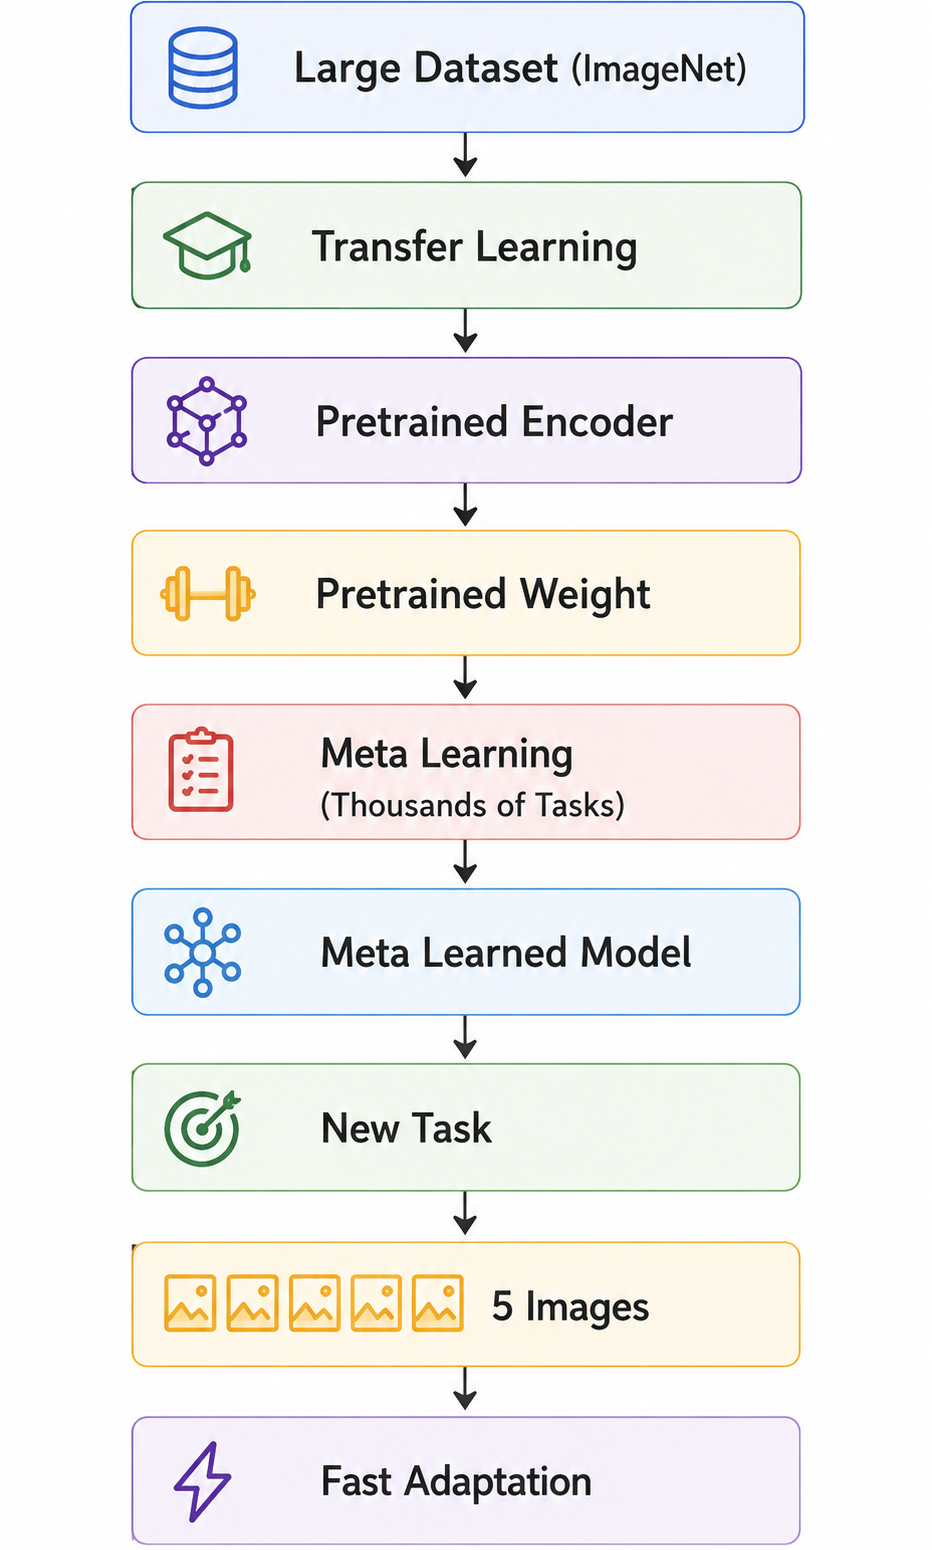
\includegraphics[width=0.95\textwidth]{figures/11-25 figure.png}
\label{fig:peft_transition}
\end{figure}

During the transfer learning stage, the backbone network learns general visual representations from a large dataset such as ImageNet. These representations capture universal image characteristics, including

\begin{itemize}
    \item edges;
    \item textures;
    \item shapes;
    \item object parts;
    \item high-level semantic concepts.
\end{itemize}

Although these pretrained features are highly informative, they are not specifically optimized for rapid adaptation to unseen tasks.

In the second stage, Meta-Learning uses the pretrained weights as the initialization for meta-training. Rather than learning visual features from scratch, the model learns how to efficiently adapt these already powerful representations to new tasks with only a few labeled examples.

By combining Transfer Learning with Meta-Learning, the resulting model benefits from both strong feature extraction and rapid adaptation, making this strategy one of the most effective approaches for modern few-shot learning systems.



